\documentclass[11pt]{aghdpl}
% \documentclass[en,11pt]{aghdpl}  % praca w języku angielskim

% Lista wszystkich języków stanowiących języki pozycji bibliograficznych użytych w pracy.
% (Zgodnie z zasadami tworzenia bibliografii każda pozycja powinna zostać utworzona zgodnie z zasadami języka, w którym dana publikacja została napisana.)
\usepackage[english,polish]{babel}

% Użyj polskiego łamania wyrazów (zamiast domyślnego angielskiego).
\usepackage{polski}

\usepackage[utf8]{inputenc}

% dodatkowe pakiety

\usepackage{mathtools}
\usepackage{amsfonts}
\usepackage{amsmath}
\usepackage{amsthm}
\usepackage{float}
\usepackage{url}
\usepackage{caption}
\usepackage{subcaption}

% --- < bibliografia > ---

\usepackage[
style=numeric,
sorting=none,
%
% Zastosuj styl wpisu bibliograficznego właściwy językowi publikacji.
language=autobib,
autolang=other,
% Zapisuj datę dostępu do strony WWW w formacie RRRR-MM-DD.
urldate=iso8601,
% Nie dodawaj numerów stron, na których występuje cytowanie.
backref=false,
% Podawaj ISBN.
isbn=true,
% Nie podawaj URL-i, o ile nie jest to konieczne.
url=false,
%
% Ustawienia związane z polskimi normami dla bibliografii.
maxbibnames=3,
% Jeżeli używamy BibTeXa:
backend=bibtex
]{biblatex}

\usepackage{csquotes}
% Ponieważ `csquotes` nie posiada polskiego stylu, można skorzystać z mocno zbliżonego stylu chorwackiego.
\DeclareQuoteAlias{croatian}{polish}

\addbibresource{bibliografia.bib}

% Nie wyświetlaj wybranych pól.
%\AtEveryBibitem{\clearfield{note}}


% ------------------------
% --- < listingi > ---

% Użyj czcionki kroju Courier.
\usepackage{courier}

\usepackage{listings}
\lstloadlanguages{TeX}

\lstset{
	literate={ą}{{\k{a}}}1
           {ć}{{\'c}}1
           {ę}{{\k{e}}}1
           {ó}{{\'o}}1
           {ń}{{\'n}}1
           {ł}{{\l{}}}1
           {ś}{{\'s}}1
           {ź}{{\'z}}1
           {ż}{{\.z}}1
           {Ą}{{\k{A}}}1
           {Ć}{{\'C}}1
           {Ę}{{\k{E}}}1
           {Ó}{{\'O}}1
           {Ń}{{\'N}}1
           {Ł}{{\L{}}}1
           {Ś}{{\'S}}1
           {Ź}{{\'Z}}1
           {Ż}{{\.Z}}1,
	basicstyle=\footnotesize\ttfamily,
}

% ------------------------

\AtBeginDocument{
	\renewcommand{\tablename}{Tabela}
	\renewcommand{\figurename}{Rys.}
}

% ------------------------
% --- < tabele > ---

\usepackage{array}
\usepackage{tabularx}
\usepackage{multirow}
\usepackage{booktabs}
\usepackage{makecell}
\usepackage{longtable}
\usepackage[flushleft]{threeparttable}

% defines the X column to use m (\parbox[c]) instead of p (`parbox[t]`)
\newcolumntype{C}[1]{>{\hsize=#1\hsize\centering\arraybackslash}X}


%---------------------------------------------------------------------------

\author{Mateusz Kuźmik}
\shortauthor{M. Kuźmik}

\titlePL{Automatyczna klasyfikacja i kategoryzacja danych tekstowych przy użyciu metod uczenia maszynowego}
\titleEN{Automatic text classification and categorization by machine learning algorithms}

\thesistype{Praca dyplomowa inżynierska}

\supervisor{dr hab. inż., prof. n. Jarosław Wąs}

\degreeprogramme{Informatyka}

\date{2019}

\department{Katedra Informatyki Stosowanej}
%\department{Department of Applied Computer Science}

\faculty{Wydział Elektrotechniki, Automatyki,\protect\\[-1mm] Informatyki i Inżynierii Biomedycznej}
%\faculty{Faculty of Electrical Engineering, Automatics, Computer Science and Biomedical Engineering}

\acknowledgements{Serdecznie dziękuję Panu dr. hab. inż. Jarosławowi Wąsowi, prof. AGH za pomoc i zaangażowanie.}

\setlength{\cftsecnumwidth}{10mm}

%---------------------------------------------------------------------------
\setcounter{secnumdepth}{4}
\brokenpenalty=10000\relax

\begin{document}

\titlepages

% Ponowne zdefiniowanie stylu `plain`, aby usunąć numer strony z pierwszej strony spisu treści i poszczególnych rozdziałów.
\fancypagestyle{plain}
{
	% Usuń nagłówek i stopkę
	\fancyhf{}
	% Usuń linie.
	\renewcommand{\headrulewidth}{0pt}
	\renewcommand{\footrulewidth}{0pt}
}

\setcounter{tocdepth}{2}
\tableofcontents
\clearpage

\chapter{Wstęp}
\label{cha:wstep}

Rozwój technologii informacyjnych przyniósł duży postęp w obszarach przetwarzania oraz przechowywania informacji. Obecnie przychodzi nam się zmagać z ogromnymi ilościami danych, z których nie jesteśmy często w stanie wyciągnąć istotnych informacji. Co więcej, w dobie internetu dane są produkowane każdego dnia oraz na bieżąco magazynowane - wymaga to coraz bardziej zaawansowanych metod, które pozwolą nam je przetworzyć.

Duża część danych jest w formie tekstu - zapisana za pomocą języka naturalnego, zrozumiałym dla człowieka. Jest to nadal duże wyzwanie dla informatyki, która nie znalazła jednoznacznej odpowiedzi na komunikację maszyny z człowiekiem. Z tego powodu odnajdywanie wartościowych informacji zapisanych za pomocą języka naturalnego jest sporym wyzwaniem w dzisiejszym świecie. Pomimo braku idealnego rozwiązania istnieje wiele skutecznych technik, opartych na algorytmach nauczania maszynowego, które postaram się w tej pracy przybliżyć.

Celem pracy jest stworzenie systemu klasyfikującego dane tekstowe. Jego model opierał się będzie na podejściu data-driven \cite{wiki:datadriven} oraz danych ogólnodostępnych w internecie. Do implementacji systemu zostaną użyte klasyczne techniki uczenia maszynowego oraz algorytmy przetwarzania tekstu naturalnego. Aplikacja zostanie wdrożona w chmurze obliczeniowej z wykorzystaniem technologii serverless \cite{Serverless}.
\chapter{Wprowadzenie teoretyczne}
\label{cha:wprowadzenieTeoretyczne}

%---------------------------------------------------------------------------

\section{Przetwarzanie języka naturalnego}
\label{sec:przetwarzanieJezykaNaturalnego}


Zgodnie z definicją, przetwarzanie języka naturalnego (zwanego dalej jako NLP - ang. Natural Language Processing) opiera się na rozpoznawaniu, rozumieniu i produkowaniu języka naturalnego. Za początki NLP uznaje się już lata pięćdziesiąte ubiegłego wieku - wtedy nastąpiła publikacją słynnego Testu Turinga. Przedstawia on sytuację w której maszyna oraz człowiek komunikują się tylko za pomocą tekstu pisanego. Turing twierdzi, że jeśli zewnętrzny obserwator po konwersacji z każdym z podmiotów nie będzie w stanie stwierdzić, który z nich jest człowiekiem - wtedy maszyna zalicza test i wykazuje zachowanie inteligentne. Pomimo wielu prób, nadal nie można jednoznacznie stwierdzić, czy jakakolwiek maszyna zaliczyła test Turinga. Podchodząc do rozwiązania wspomnianego testu, nietrudno wywnioskować jest, że kluczem do jego rozwiązania będzie rozumienie języka naturalnego (ludzkiego) przez maszynę. 

Przez ponad 30 lat od definicji Testu Turinga rozwiązywanie problemów NLP bazowane było na złożonych zasadach definiowanych ręcznie w algorytmach. Dopiero lata 80’ przyniosły znaczny postęp w tej dziedzinie. W związku z wzrostem mocy obliczeniowej komputerów zaczęto używać metod uczenia maszynowego, które pozwalały na uzyskanie dużo lepszych wyników w rozwiązywaniu tych problemów. Jednym z modeli wykorzystywanych na początku było drzewo decyzyjne, które skutkowało w produkcji modelu złożonego z wielu instrukcji warunkowych, co miało wiele podobieństw z modelami bazującymi na definiowaniu zasad używanymi przed erą uczenia maszynowego w problemach NLP. Jednakże użycie tych metod pozwalało na automatyzację procesu tworzenia modelu, co znacznie ułatwiło dalszy rozwój. Od tego momentu duża część aplikacji i rozwiązań zbudowanych wokół problemu NLP opiera się na podejściu data-driven.

Problem NLP stał się również bardzo znaczący w kontekście powstania i rozwoju Internetu. W Internecie z upływem czasu znajduje się coraz więcej danych, z których ogromną ilość stanowią dane w formie tekstu. Rozwój metod NLP pozwala nam na efektywne przeszukiwanie zasobów w sieci. Działa to również w drugą stronę: dane pochodzące z Internetu są wykorzystywane do uczenia algorytmów NLP, co sprawia, że zasoby w sieci są coraz szybciej dostępne i lepiej uporządkowane.

W kolejnych podrozdziałach skupię się na opisach oraz analizie metod NLP w kontekście dużych zbiorów danych oraz podejściu data-driven.

\subsection{Zbieranie danych}

Pierwszą i niezbędną częścią tworzenia systemu rozwiązującego problem przetwarzania języka naturalnego podejściem data-driven jest zbieranie danych tekstowych. Ważnym aspektem tutaj jest jakość oraz ilość zebranych danych - będą one znacząco wpływać na skuteczność rozwiązania problemu. Idealny zbiór danych powinien zawierać reprezentatywne dane, jasno podzielone na kategorie/gatunki i w podobnej ilości dla każdej kategorii. Ta ostatnia cecha może stanowić spory problem przy budowaniu zbioru danych. Przykładowo budując system przypisujący dziedzinę nauki do wprowadzonego artykułu naukowego musimy zebrać dostateczną ilość reprezentatywnych artykułów oznaczonych konkretną dziedziną jakiej dotyczą. Musimy się liczyć z różną dostępnością artykułów z poszczególnych dziedzin. Rozwiązaniem jest odrzucenie części artykułów i zebranie dla każdej dziedziny tylko tylu, ile możemy znaleźć dla dziedziny z najmniejszą ilością artykułów, przy czym musimy pamiętać, że wielkość zestawu ma duży wpływ na skuteczność systemu.

Dane mogą być zbierane zarówno drogą manualną, jak i automatyczną. W celu pozyskania zbioru o wysokiej jakości często niezbędne jest zatrudnianie ekspertów z dziedziny lingwistyki, którzy własnoręcznie gromadzą i opisują dane. Obecnie raczej dużo częściej wykorzystywane są metody automatyczne, głównie ze względu na ilość danych jakie potrafią zgromadzić. Projekty osobistych asystentów (Apple Siri, Google Assistant itp.) i ich sukces dowodzą, że dane zebrane metodami automatycznymi znakomicie sprawdzają się przy uczeniu maszynowym i poleganie jedynie na metodach manualnych nie jest konieczne.

Unikniemy wielu problemów związanych z zbieraniem danych, jeśli wykorzystamy gotowe zestawy dostępne w sieci. Przykładem jest British National Corpus - posiada on wiele przykładów tekstu z gazet, magazynów, tekstów akademickich i innych rzetelnych źródeł. Każdy tekst podzielony jest na słowa z których każde jest oznaczone właściwą częścią mowy, formą i innymi parametrami zgodnymi ze standardem TEI \footnote{http://www.tei-c.org/}.


\subsection{Analiza i przetwarzanie danych}

Po etapie pozyskania danych bardzo ważnym procesem jest ich przetworzenie i właściwe oznaczenie. W obecnych czasach wykorzystuje się do tego raczej automatyczne narzędzia, które znacznie ograniczają czas i wysiłek włożony w cały proces przetwarzania języka naturalnego.

Przykładowe procesy stosowane przy przetwarzaniu tekstu:
\begin{enumerate}
    \item Lematyzacja lub stemming - ich celem jest mapowanie słowa z tekstu na ich formę kanoniczną. Jako rezultat słowa o takim samym znaczeniu, ale innej formie traktowane są jako jedno i to samo. Proces ten często prowadzi do utraty części informacji zawartych w tekście, lecz pozwala na prostsze przetwarzanie danych w dalszych etapach.

    \newpage
    \begin{lstlisting}[caption={Przykład lematyzacji},captionpos=b]
        are, be, am, is => be
        analyse, analysis, analyses => analyse
    \end{lstlisting}
    
    \item Tagowanie części mowy (ang. Part-of-speech tagging) - oznaczanie każdego wyrazu z jego częścią mowy.

    \begin{lstlisting}[caption={Przykład tagowania części mowy}]
        James => noun
        made => verb
    \end{lstlisting}
    
    \item Parsowanie - podobnie do parsowania języka programowania - tutaj także budujemy drzewo syntaktyczne ze zdania w języku naturalnym. Jest ono trudniejszym procesem od dwóch poprzednich, ponieważ wymaga bardziej zaawansowanej wiedzy z dziedziny lingwistyki.

    \begin{figure}[H]
    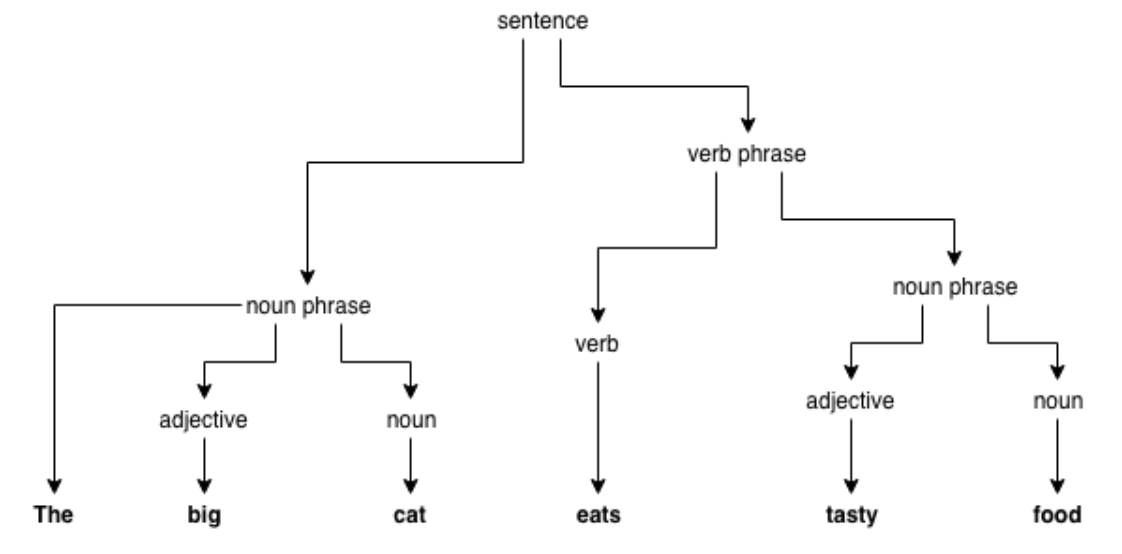
\includegraphics[width=10cm]{parsing_example.png}
    \centering
    \caption{Przykład parsowania zdania}
    \end{figure} 
    
\end{enumerate}

Wstępnie przetworzony tekst jest łatwiejszy do analizy - niektóre z popularnych metod analizy tekstu to:

\begin{enumerate}
    \item Zgodność (ang. concordance) - badanie kontekstu danego słowa. Jako rezultat dostajemy różne otoczenia w jakich słowo występuje w zbiorze danych.
    
    \item Częstość występowania słowa - uzyskanie listy najczęściej występujących słów w naszym zbiorze.

    \item Szukanie sekwencji słów które często występują obok siebie (ang. collocation extraction).

\end{enumerate}

\subsubsection{N-gram}

N-gramem jest nazywana sekwencja kolejnych n elementów występujących po sobie w przetwarzanej próbce. W przypadku przetwarzania języka naturalnego najczęściej bierze się pod uwagę kolejne słowa. Dzięki analizie n-gramów znamy kontekst występowania danego słowa, lub jesteśmy w stanie przewidzieć jakie słowo może pojawić się dalej. Weźmy pod uwagę przykładowe zdanie: “to be or not to be”. Rozkład na modele n-gram może wyglądać następująco:

\begin{enumerate}
    \item unigramy: [ ‘to’, ‘be’, ‘or’, ‘not’, ‘to’, ‘be’ ] 
    \item bigramy: [ ‘to be’, ‘be or’, ‘or not’, ‘not to’, ‘to be’ ]
    \item trigramy: [‘to be or’, ‘be or not’, ‘or not to’, ‘not to be’ ]
\end{enumerate}

Przy przetwarzaniu tekstu n-gramy wydają się bardzo przydatnym modelem pod kątem analizy kontekstu. Polegając jedynie na unigramach nie będziemy w stanie wyciągnąć wielu znaczących informacji z tekstu takich jak negacje  (‘good’ vs ‘not good’) lub zaprzeczenia (‘do’ vs ‘do not’).

\subsubsection{Bag of words}

Aby umożliwić przetwarzanie tekstu przez algorytmy uczenia maszynowego trzeba sprowadzić go do reprezentacji macierzowej. Bag of words jest jednym z najprostszych modeli pozwalających wykonać to zadanie. Każdy element macierzy wyprodukowanej przez ten model odpowiada liczbie wystąpień jednego słowa z tekstu.

\begin{verbatim}
    Dane wejściowe: “Machine learning gains more and more popularity.”
    Bag of words: { 
        “machine”: 1, 
        “learning”: 1, 
        “gains”: 1, 
        “more”: 2, 
        “and”: 1, 
        “popularity”: 1 
    }
\end{verbatim}

\subsubsection{TF-IDF}

Rozszerzeniem modelu Bag of words jest Term Frequency - Inverse Document Frequency \footnote{https://pl.wikipedia.org/wiki/TFIDF}. Do klasycznego Bag of words dodaje on wagę do każdego ze słów. Słowo często występujące w jednym dokumencie, a rzadko w innych będzie miało wyższą wagę, natomiast słowo występujące równie często w analizowanym dokumencie, w reszcie zostanie oznaczone niższą wagą.

%---------------------------------------------------------------------------

\section{Uczenie maszynowe}
\label{sec:uczenieMaszynowe}

Algorytmy uczenia maszynowego pozwalają nam na tworzenie rozwiązań bazujących na doświadczeniach i przykładach, zamiast na jawnie zaprogramowanych zasadach. Algorytmy uczenia maszynowego wymagają często większej mocy obliczeniowej niż standardowe rozwiązania, ponieważ bazują na dużych zestawach danych wejściowych. 

Rodzaje algorytmów uczenia maszynowego:

\begin{enumerate}
    \item Uczenie nadzorowane - zasilane przez opisane dane na podstawie których algorytm jest uczony i dopiero po wykonaniu tego procesu jest on gotowy do użycia.

    \item Uczenie nienadzorowane - algorytmy zasilane są nieopisanymi danymi, które mają uporządkować poprzez znalezienie podobnych cech pośród danych wejściowych.
\end{enumerate}

Przykład: Na podstawie rozmiaru buta i wzrostu mamy zadanie określić płeć człowieka.
W uczeniu nadzorowanym wizualizacja zestawu danych może wyglądać następująco:

    \begin{figure}[H]
    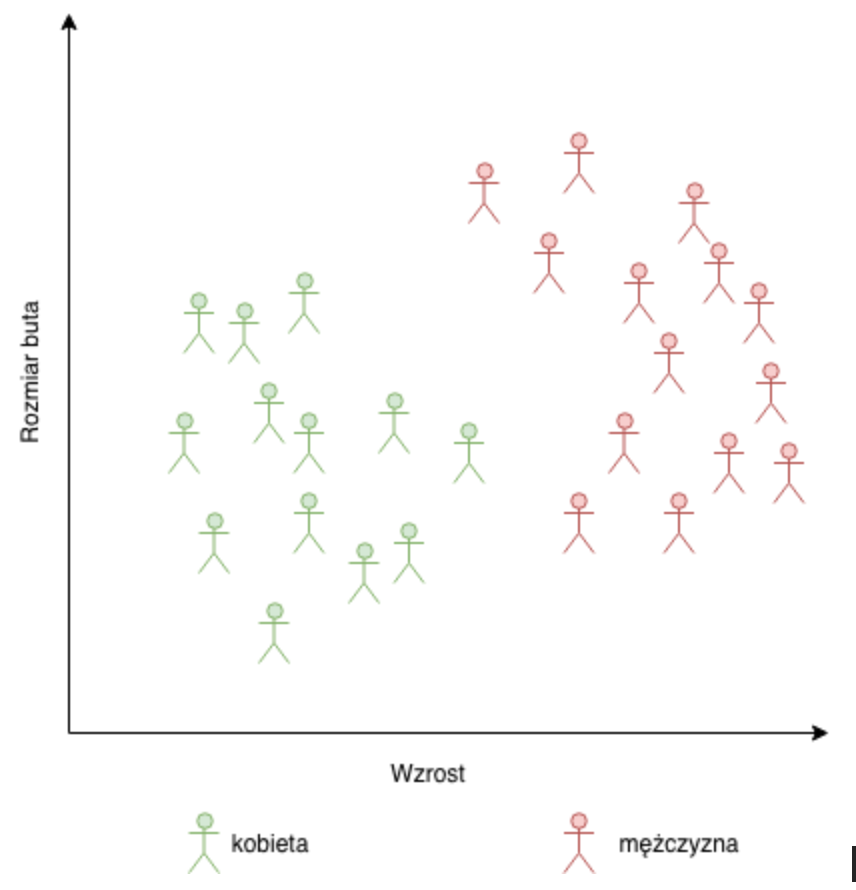
\includegraphics[width=8cm]{supervised_dataset_example.png}
    \centering
    \caption{Wizualizacja przykładowego zbioru uczącego w uczeniu nadzorowanym}
    \end{figure}
    
Wykorzystując algorytm uczenia nienadzorowanego, nasze dane nie są opisane. W podanym przykładzie możemy wykorzystać automatyczną klasteryzację.

    \begin{figure}[H]
    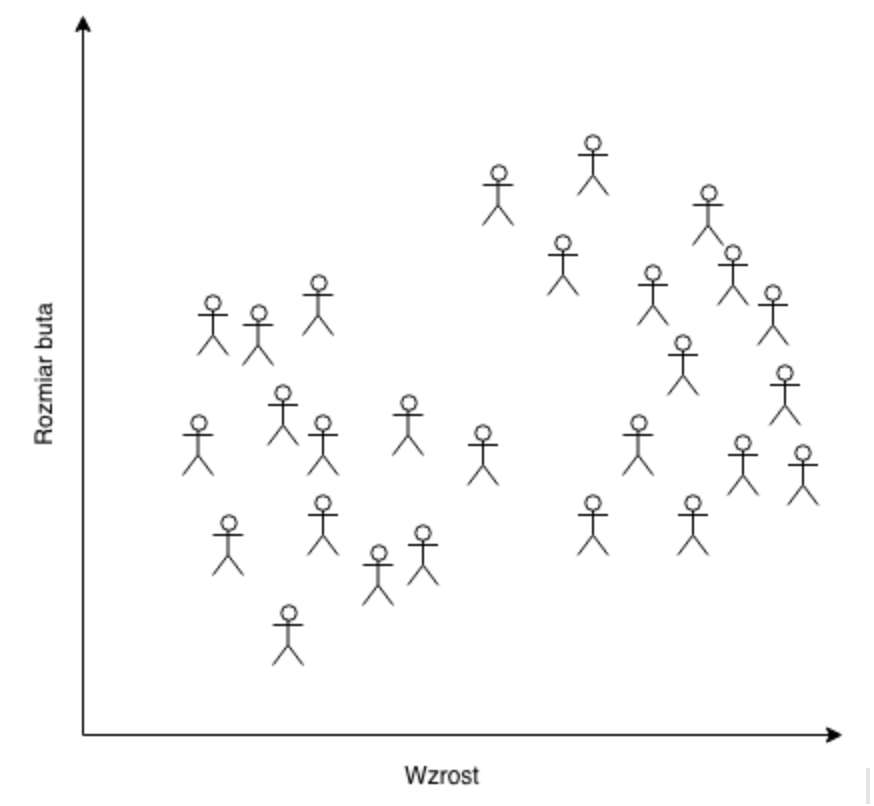
\includegraphics[width=8cm]{unsupervised_dataset_example.png}
    \centering
    \caption{Wizualizacja przykładowego zbioru w uczeniu nienadzorowanym}
    \end{figure}
    
Obszar uczenia nadzorowanego możemy podzielić również na zastosowania:
\begin{enumerate}
    \item Regresja - obszar uczenia nadzorowanego, w którym dane wyjściowe mają postać ciągłą. Przykład - oszacowanie ceny mieszkania na podstawie odległości od centrum miasta:
    
    \begin{figure}[H]
    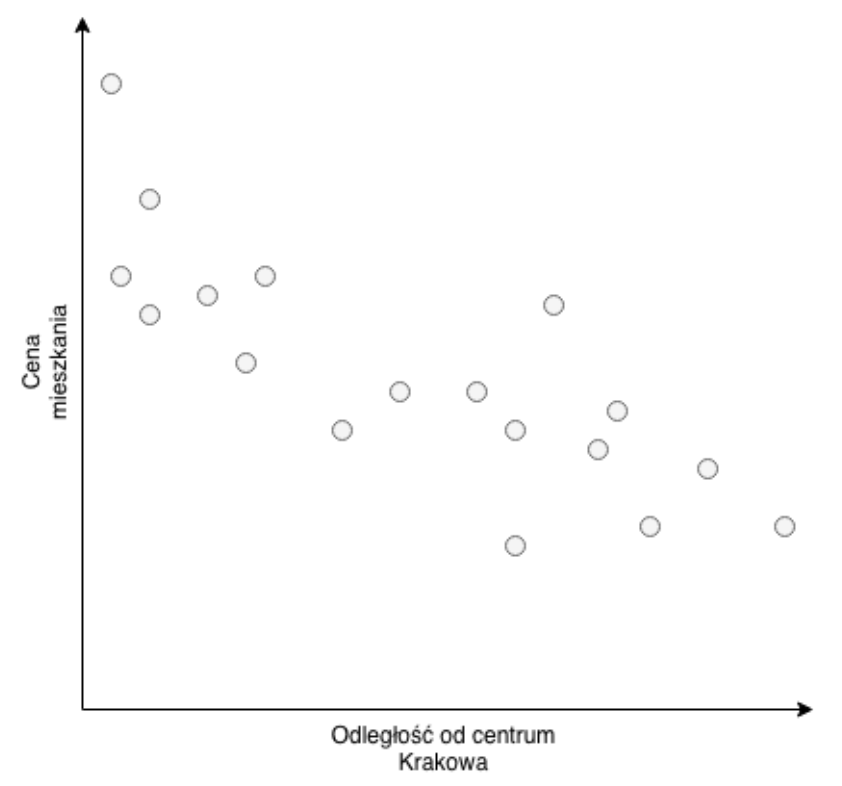
\includegraphics[width=8cm]{regression_dataset_example.png}
    \centering
    \caption{Wizualizacja przykładowego zbioru uczącego w problemie regresji}
    \end{figure}
    
    \item Klasyfikacja - należy również do uczenia nadzorowanego. Dane wyjściowe w problemach klasyfikacji mają postać dyskretną. Przykład: klasyfikacja nowotworu według wielkości guza.
    
    \begin{figure}[H]
    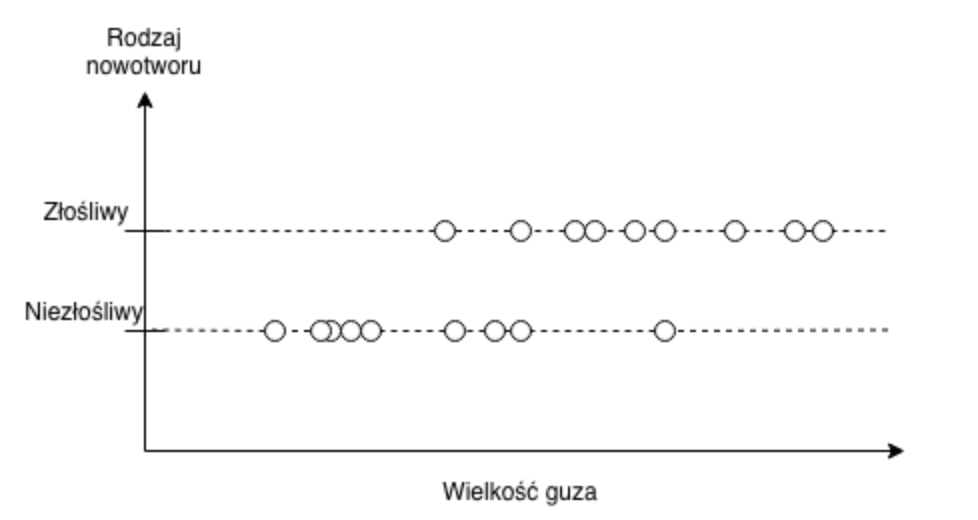
\includegraphics[width=8cm]{classification_dataset_example.png}
    \centering
    \caption{Wizualizacja przykładowego zbioru uczącego w problemie klasyfikacji}
    \end{figure}    
    
    \item Klasteryzacja - problem związany z uczeniem nienadzorowanym. Algorytm sam znajduje strukturę wprowadzonych danych i próbuje je rozdzielić na określoną (manualnie lub dynamicznie) liczbę klastrów.
    
    \begin{figure}[H]
    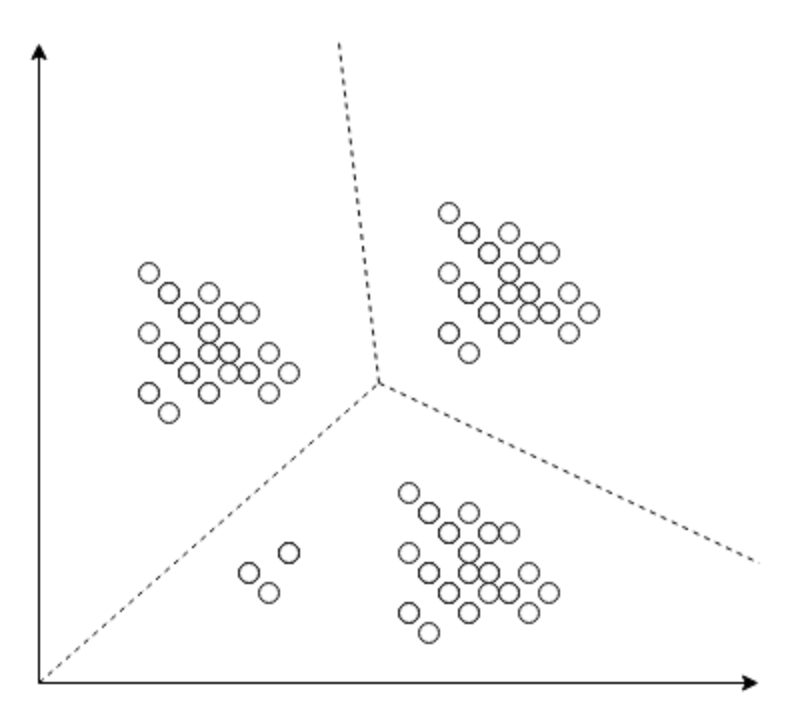
\includegraphics[width=8cm]{clustering_example.png}
    \centering
    \caption{Wizualizacja przykładowego procesu klasteryzacji}
    \end{figure}
    
\end{enumerate}

\subsection{Wybrane algorytmy uczenia maszynowego}

\subsubsection{Naiwny klasyfikator bayesowski}

Naiwny klasyfikator bayesowski jest oparty na metodach statystycznych, a dokładniej twierdzeniu Bayesa. Metoda ta zakłada, że wszystkie atrybuty (cechy) próbki mają być od siebie niezależne.

\textbf{Założenia}: Zbiór uczący składa się z n próbek, z których każda ma po m atrybutów. Każda próbka w zbiorze uczącym musi mieć również przypisaną klasę ze zbioru skończonego C. Posiadamy również jedną próbkę (określmy ją jako X) opisaną również przez m atrybutów (takich samych jak w zbiorze uczącym). Naszym zadaniem jest przypisanie odpowiedniej klasy ze zbioru C do próbki X.

\[ P(C_i|X) = \frac{P(X|C_i)P(C_i)}{P(X)} \]

\begin{center}
    $P(C_i|X)$ - prawdopodobieństwo, że X należy do klasy Ci
\end{center}

$P(X)$ jest dla wszystkich kategorii równe, dlatego możemy wykluczyć je z algorytmu.
Zakładamy również, że poszczególne kategorie mają równe prawdopodobieństwa 
$(C1 = C2 = ... = Cz)$, dzięki czemu nasze zadanie sprowadza się do maksymalizacji $P(X|C_i)$.

Wcześniej poczynione założenie mówiące, że wszystkie atrybuty są od siebie niezależne pozwala nam na kolejne przekształcenie równania do postaci:

\[ P(C_i|X) = \prod^{m}_{k=1} P(X_k|C_i) \]

Na tej podstawie jesteśmy już w stanie policzyć $P(Xk|C_i)$:

\begin{enumerate}
    \item Jeśli atrybut $X_k$ ma wartość ze zbioru skończonego (np. jest kategorią), wtedy liczymy prawdopodobieństwo, że próbki testowe należące do Ci mają atrybut k taki sam jak próbka X
    
    \item Jeśli atrybut jest wartością ciągłą, wtedy powinniśmy obliczyć $P(X_i|C)$ korzystając z funkcji rozkładu Gaussa.
\end{enumerate}

Wartość $P(C_i|X)$ musimy policzyć dla każdej klasy. Klasa dla której prawdopodobieństwo będzie największe, stanie się potencjalną kategorią próbki X.

Dużymi zaletami klasyfikatora Bayesa jest niska złożoność obliczeniowa i prostota. Natomiast należy cały czas pamiętać, że ten klasyfikator nie będzie dawał dobrych rezultatów, jeśli będą występowały znaczące zależności między atrybutami.

\subsection{Metoda k-średnich}

W problemach klasteryzacji jednym z najpopularniejszych obecnie algorytmów jest metoda k-średnich. Jego głównymi atutami są prostota oraz efektywność. Algorytm składa się z trzech ogólnych kroków:

\begin{enumerate}
    \item Inicjalizacja k centroidów (gdzie k jest dowolną liczbą całkowitą większą od zera).
    
    \item Przypisanie każdej próbki do jej najbliższego centroidu.

    \item Zmień pozycję centroidów biorąc po uwagę przypisania z punktu 2 (ustalona zostaje jako średnia wszystkich punktów przypisanych do centroidu). Jeśli pozycja się nie zmienia, zakończ działanie.
\end{enumerate}

Złożoność obliczeniową algorytmu k-means przyjmuje się jako: 

\[ O(t * k * n * d) \]

\begin{center}
t - ilość iteracji

k - ilość klastrów

n - ilość próbek

d - liczba wymiarów (dla pojedynczej próbki)
\end{center}

Pomimo liniowej złożoności algorytm k-średnich ma problemy z dużymi ilościami danych pochodzących z internetu, gdzie ilości próbek, klastrów oraz wymiarów są ogromne. Kolejnym problemem jest inicjalizacja klastrów. Wynik końcowy może się różnić w zależności od pierwotnych położeń centroidów.

\begin{figure}[H]
    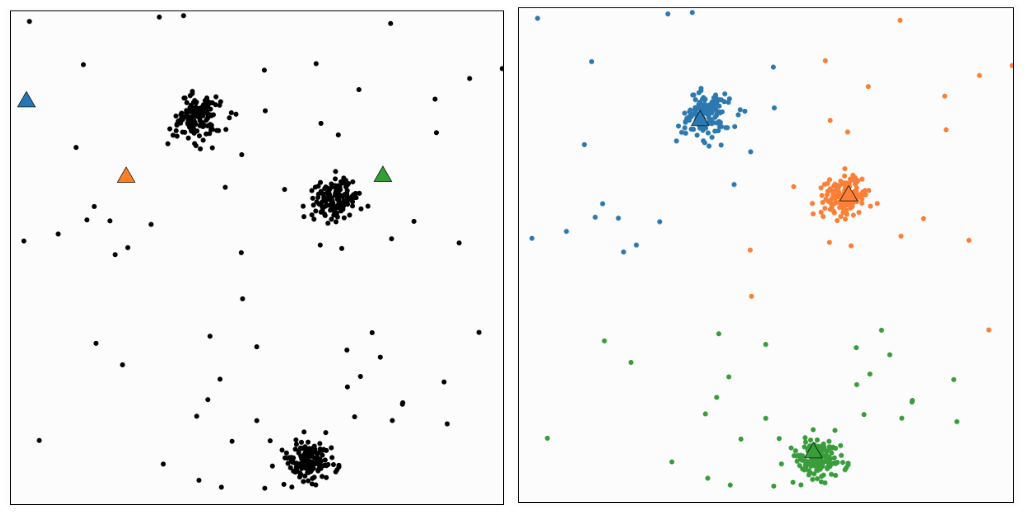
\includegraphics[width=10cm]{kmeans_example.png}
    \centering
    \caption{Przykład klasteryzacji (przed i po 8 iteracjach) na podstawie https://github.com/karanveerm/kmeans}
\end{figure} 

\chapter{Wprowadzenie technologiczne}
\label{cha:wprowadzenieTechnologiczne}

%---------------------------------------------------------------------------

\section{DynamoDB}
\label{sec:dynamoDb}


Do aplikacji, które wykorzystują podejście data-driven trzeba wykorzystywać bazy danych, które pozwalają na przechowywanie i zarządzanie dużymi ilościami danych. Takie aplikacje rzadko mają skomplikowany model, zwykle składa się on z niewielu tabel, które zawierają bardzo duże ilości rekordów.

Amazon DynamoDB to system bazodanowy rozproszony pomiędzy wieloma partycjami oferujący wysoką wydajność. Dużym atutem tego systemu jest skalowalność, ponieważ jesteśmy w stanie dodawać nowe maszyny do klastra w trakcie działania systemu. Jest to możliwe, ponieważ każdy wiersz w tabeli ma określoną maszynę na której się znajduje poprzez wyliczenie jego skrótu (ang. hash) algorytmem “Consistent hashing”.  Dane rozłożone na wielu maszynach są szybciej dostępne oraz bezpieczniejsze, ponieważ w całym systemie nie ma pojedynczego punktu, który mógłby spowodować awarię całej bazy danych.


Kluczowe cechy DynamoDB:

\begin{enumerate}
    \item Brak jednoznacznej struktury w tabeli.

Podobnie jak w relacyjnej bazie danych - struktura DynamoDB składa się z tabel, które zawierają rekordy (DynamoDB nie nakłada limitu na liczbę rekordów w tabeli, barierą jest jedynie pamięć fizyczna). W odróżnieniu od systemów relacyjnych - rekordy w DynamoDB nie posiadają ustalonej struktury. Jedyną rzeczą jaką musi posiadać dany rekord jest Partition Key.

    \item Rozproszenie danych.

DynamoDB może przechowywać dane w obrębie jednej tabeli na kilku fizycznych maszynach - jest to możliwe dzięki Partition Key używany jest on jako argument funkcji haszującej, której wynik decyduje na której maszynie znajdzie się rekord. Konsekwencją jest to, że szukając jakichkolwiek danych musimy znać ich Partition Key lub mieć stworzony indeks na innym atrybucie - w przeciwieństwie do klasycznych systemów relacyjych, zapytania wykorzystujące dowolny atrybut jako warunek nie są dozwolone.

    \begin{figure}[H]
    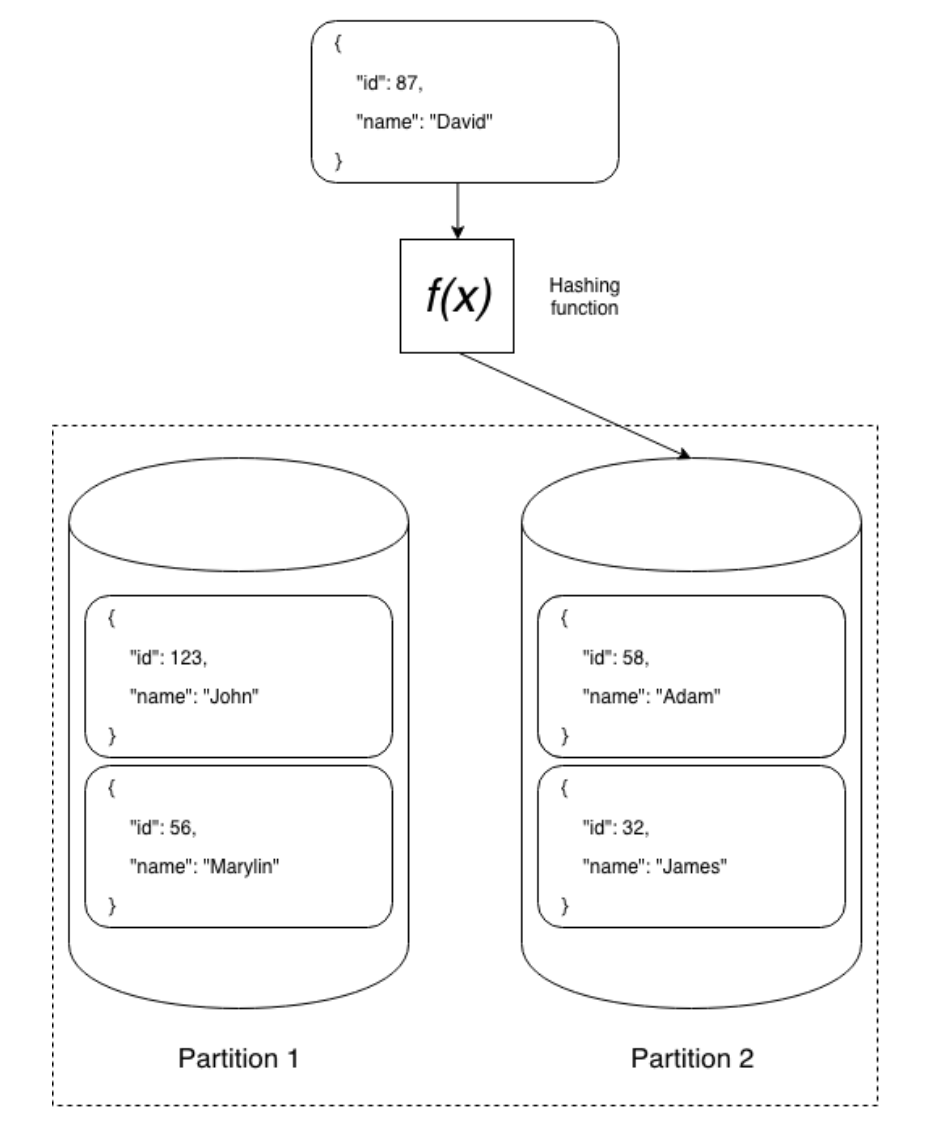
\includegraphics[width=11cm]{dynamo_partitions.png}
    \centering
    \caption{Schemat umieszczania rekordu w DynamoDB}
    \end{figure} 

    \item Eventual/Strong Consistency.

System bazodanowy DynamoDB pozwala nam na działanie w dwóch poziomach konsystencji. Strong consistency pozwala nam na odczytanie najbardziej aktualnych danych znajdujących się w systemie. Ma on jedno ważne wymaganie - wszystkie maszyny w systemie muszą być sprawne (co w systemach rozproszonych nie jest wcale oczywiste). Mamy też drugi poziom bardziej odpowiadający charakterystyce systemów rozproszonych - Eventual consistency. W tym trybie istnieje ryzyko otrzymania nieaktualnych danych - natomiast zapewnione jest, że jeśli powtórzymy zapytanie po pewnym czasie, dane zostaną uaktualnione. Czas ten jest inny dla każdego systemu - zależy on od szybkości replikacji danych.

    \item Skalowalność horyzontalna.

Im więcej danych przechowujemy, tym więcej partycji je przechowuje. Zwiększanie rozmiarów tabeli nie wpływa na wydajność kwerend wykonywanych na nich. 

    \item “No single point of failure”

Dzięki zastosowaniu wielu partycji, z których każda działa niezależnie - system jest częściowo odporny na awarie. Nasze dane nie są przechowywane na jednej maszynie, dzięki czemu nie grozi nam całkowita utrata przechowywanych danych.
\end{enumerate}


\section{Serverless}
\label{sec:serverless}

W ostatnich latach technologie “serverless” zyskały dużą popularność wraz z rozwojem chmur obliczeniowych. Ta technologia jest znana także jako FaaS (function as a service), ponieważ dostawca usług chmurowych zapewnia nam całą infrastrukturę oraz zarządzanie nią, podczas gdy my (jako klienci) musimy dostarczyć tylko funkcję (kod programu), jaka będzie wykonywana podczas zapytania do usługi. Wybrane zalety usług “serverless” to:

\begin{enumerate}
    \item Skalowalność - funkcja  wdrożona w środowisku serverless może w nim przebywać nie generując kosztów jeśli nie jest ona wywoływana. Z drugiej strony, gdy mamy do czynienia z dużym ruchem - infrastruktura wykonująca nasze funkcje jest skalowana horyzontalnie, dzięki czemu infrastruktura nie jest ograniczeniem wydajności aplikacji.
    
    \item Czas potrzebny od napisania kodu do uruchomienia go na serwerze jest dużo mniejszy niż przy użyciu infrastruktury on-premise. Cała konfiguracja oraz zarządzanie środowiskiem jest odpowiedzialnością dostawcy usług chmurowych.
\end{enumerate}

Pomimo zalet trzeba również pamiętać o innych cechach tych usług, które trzeba wziąć po uwagę, gdy planujemy tworzyć aplikację pod kątem działania jako serverless:

\begin{enumerate}
    \item “Cold start” - jest to czas potrzebny na uruchomienie środowiska aplikacji. Jeśli nasza funkcja nie jest wywoływana przez dany czas, jej środowisko zostaje wyłączone, przez co pierwsze wywołanie po takim czasie zajmuje znacznie więcej czasu niż pozostałe. Efekt ten jest zależny od czasu startu oraz pamięci wymaganej przez aplikację, czyli w C# oraz Java będzie on znacznie bardziej uciążliwy niż dla funkcji zaimplementowanych w Python.3

    \item Przetwarzanie długich zapytań - większość dostawców usług “serverless” ma limity czasowe na wykonanie jednego wywołania funkcji. Każdy proces, który zajmie dłużej jest natychmiast zakończony. Aplikacje, posiadające takie cechy potrzebują poważnych zmian w architekturze zanim zostaną przeniesione na usługi “serverless”.
\end{enumerate}

\chapter{Analiza danych oraz test algorytmów}
\label{cha:analizaDanych}

Prace nad systemem kategoryzacji zacząłem od wyboru danych na których będę bazował. Wybór padł na dane z obszaru newsów - jego motywacją był jasny podział na kategorie. Niemal w każdym przypadku człowiek jest w stanie odróżnić wiadomość sportową od wiadomości ze świata biznesu. Dodatkowym atutem była jakość danych znajdujących się w internecie. Każdy news ze znanych portali informacyjnych ma jasno przypisaną kategorię oraz zazwyczaj jego zawartość jest dobrej jakości - nie zawiera kolokwialnego języka, błędów ortograficznych oraz literówek, które utrudniałyby jego przetwarzanie. Dla ułatwienia projektu skupiłem się na danych w języku angielskim - z powodu jego popularności jest on obecnie językiem, który najłatwiej poddaje się przetwarzaniu maszynowemu.

Po wstępnym zebraniu danych zamierzałem wyciągnąć z nich informacje stosując następujące kroki:

\begin{enumerate}
    \item Wstępne przetworzenie danych tekstowych.
    \item Sprowadzenie ich do modelu Bag Of Words oraz TF-IDF.
    \item Podzielenie danych na zbiór uczący i testowy.
    \item Sprawdzenie skuteczności różnych algorytmów nadzorowanego uczenia maszynowego na zebranych danych.
\end{enumerate}

%---------------------------------------------------------------------------

\section{Gromadzenie danych}
\label{sec:gromadzenieDanych}

Pierwszy zestaw newsów do analizy pochodził ze źródła www.inshorts.com, w którym możemy znaleźć wiadomości z różnych kategorii z których każdy ma długość około 60 słów. Struktura pobranych danych składała się z dwóch elementów - zawartości newsa (content) oraz etykiety opisującej go (label).

    \begin{figure}[H]
    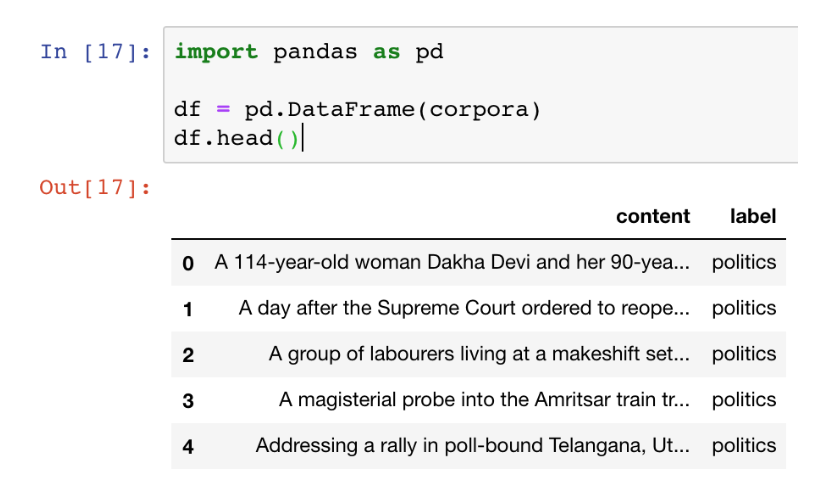
\includegraphics[width=8cm]{content_example.png}
    \centering
    \caption{Przykład zebranych danych.}
    \end{figure} 
    
Histogram ilości słów dla 2657 newsów:

    \begin{figure}[H]
    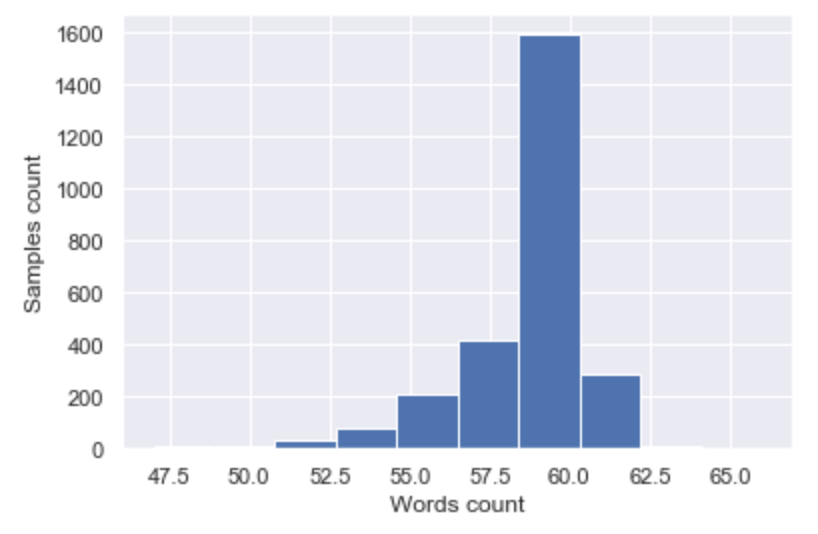
\includegraphics[width=8cm]{words_count.png}
    \centering
    \caption{Histogram ilości słów w tekście}
    \end{figure} 

\section{Wstępne przetwarzanie danych}

Surowe dane tekstowe pobrane z internetu nie do końca nadają się do użycia w algorytmach uczenia maszynowego. Zawierają one znaki interpunkcyjne, duże litery, stop-słowa \footnote{https://www.seopilot.pl/wiki/Stopwords.html} oraz te same wyrazy w różnej formie gramatycznej. Aby ułatwić analizę danych oraz uczenie algorytmów zastosowałem kilka kroków przetwarzania wstępnego danych w celu ich uproszczenia:

\begin{enumerate}
    \item Zamiana wielkich liter na małe.
    \item Usunięcie znaków interpunkcyjnych oraz cyfr.
    \item Zamiana wszystkich znaków na znaki występujące w zbiorze ASCII.
    \item Lematyzacja, czyli sprowadzenie słów do ich podstawowych form gramatycznych.
    \item Usunięcie stop-słów.
\end{enumerate}

\newpage
Przykładowy tekst przed i po przetworzeniu:

\begin{verbatim}
    TEKST WEJŚCIOWY: 
    There’s been a lot written about the theory behind TF-IDF but the 
    gist is: calculate the term frequency (TF), or number of times 
    a word appears across the text you’re interested in analysing.
    This is intuitive - more important words appear 
    more often right?
    
    TEKST WYJŚCIOWY: 
    lot written theory behind tfidf gist calculate term frequency
    tf number time word appears across text youre interested
    analysing intuitive important word appear often right
\end{verbatim}

Aby lepiej zrozumieć istotę przetwarzania wstępnego danych tekstowych, na wykresie \ref{wykr:slowa_bez_pre} widać 10 najczęściej występujących słów we wszystkich zebranych newsach. Są to głównie słowa nie niosące za sobą konkretnej informacji, które mogą wpływać negatywnie na sprawność algorytmów uczenia maszynowego. 

    \begin{figure}[H]
    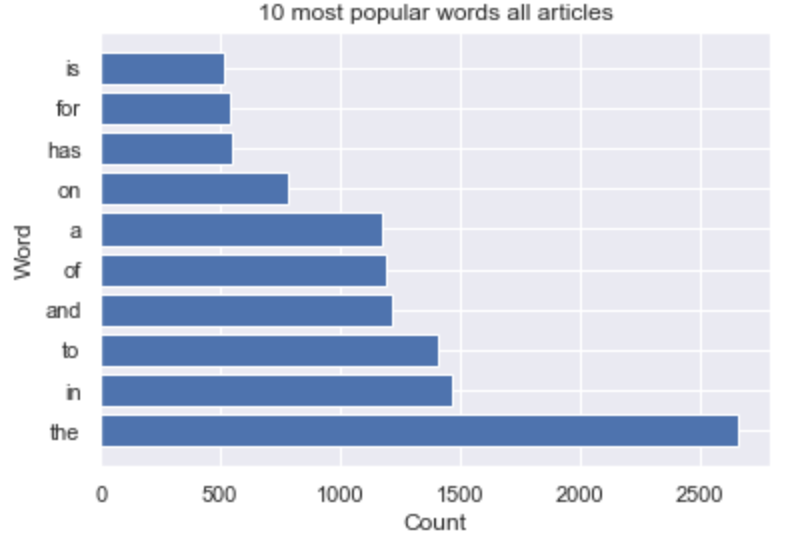
\includegraphics[width=8cm]{images/analiza/all_unprocessed.png}
    \centering
    \caption{10 najpopularniejszych słów w całym korpusie bez zastosowania wstępnego przetwarzania.}
    \label{wykr:slowa_bez_pre}
    \end{figure} 

\section{Wizualizacja danych}

Po przetworzeniu tekstu możemy go poddać analizie częstotliwości występowania słów w każdej kategorii. Na wykresach \ref{fig:10_most_popular_words} widać wyraźnie, że zestawy słów różnią się pomiędzy sobą. Słowa które się powtarzają to są czasownikami charakterystycznymi dla newsów (said, have, was itp.). Z występowania tych słów również można wyciągnąć ciekawe wnioski. Na przykład duża popularność słowa 'said' w kategorii rozrywka może świadczyć o dużej ilości cytatów w artykułach z tej kategorii.

\begin{figure}[H]
     \centering
     \begin{subfigure}[b]{0.7\textwidth}
         \centering
         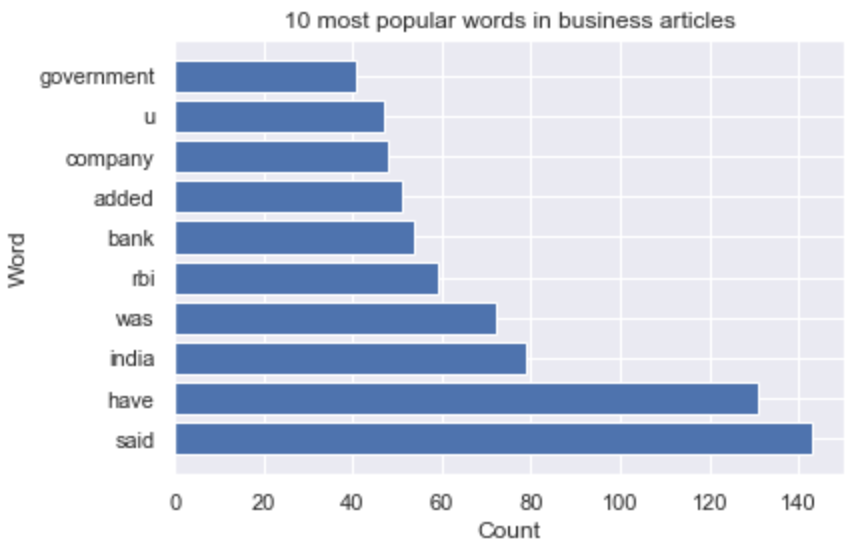
\includegraphics[width=\textwidth]{images/analiza/business.png}
     \end{subfigure}
     \hfill
     \begin{subfigure}[b]{0.7\textwidth}
         \centering
         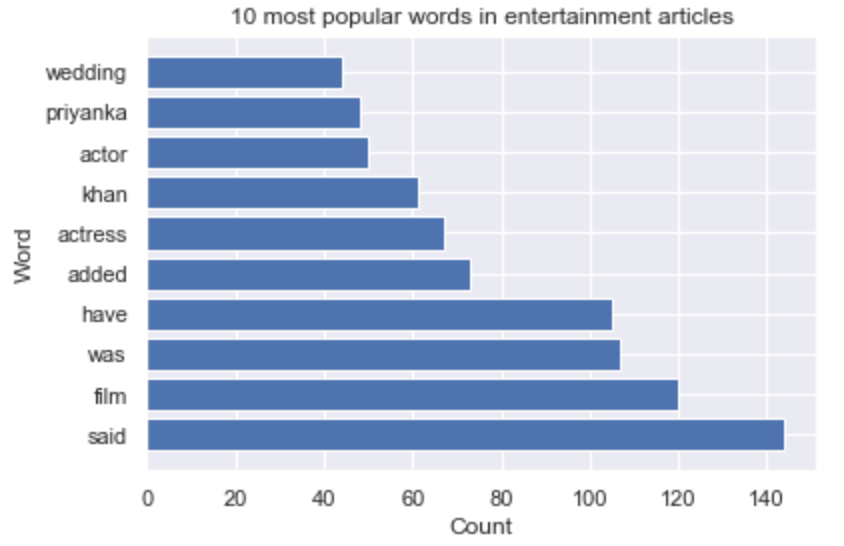
\includegraphics[width=\textwidth]{images/analiza/entertainment.png}
     \end{subfigure}
     \hfill
     \begin{subfigure}[b]{0.7\textwidth}
         \centering
         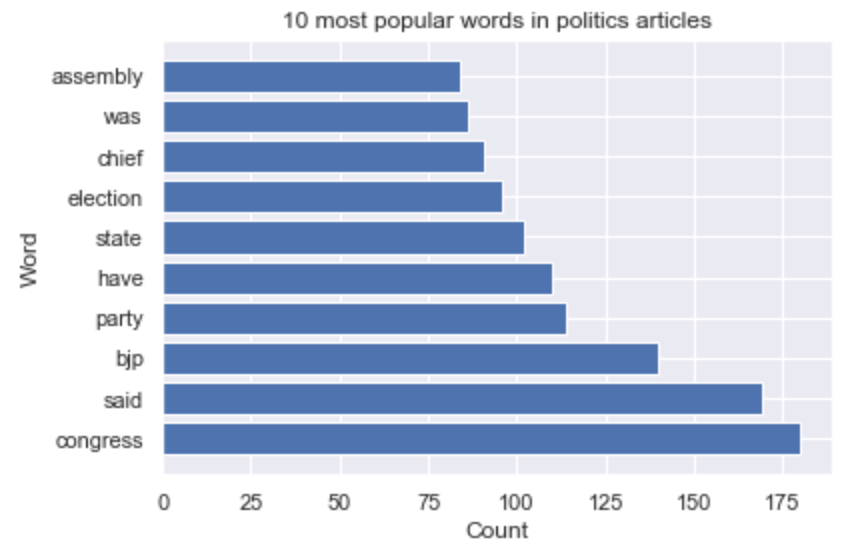
\includegraphics[width=\textwidth]{images/analiza/politics.png}
     \end{subfigure}
\end{figure}
\begin{figure}[H]\ContinuedFloat                 \begin{subfigure}[b]{0.7\textwidth}
         \centering
         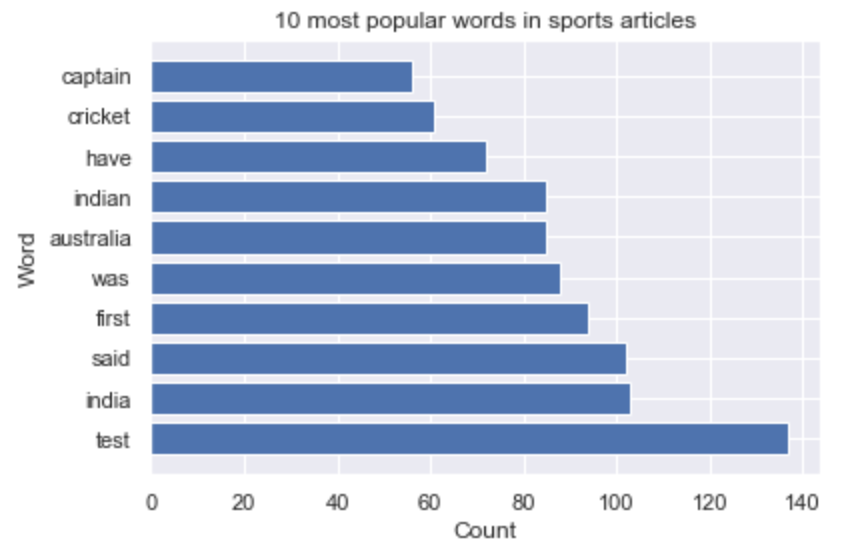
\includegraphics[width=\textwidth]{images/analiza/sports.png}
     \end{subfigure}
     \hfill
     \begin{subfigure}[b]{0.7\textwidth}
         \centering
         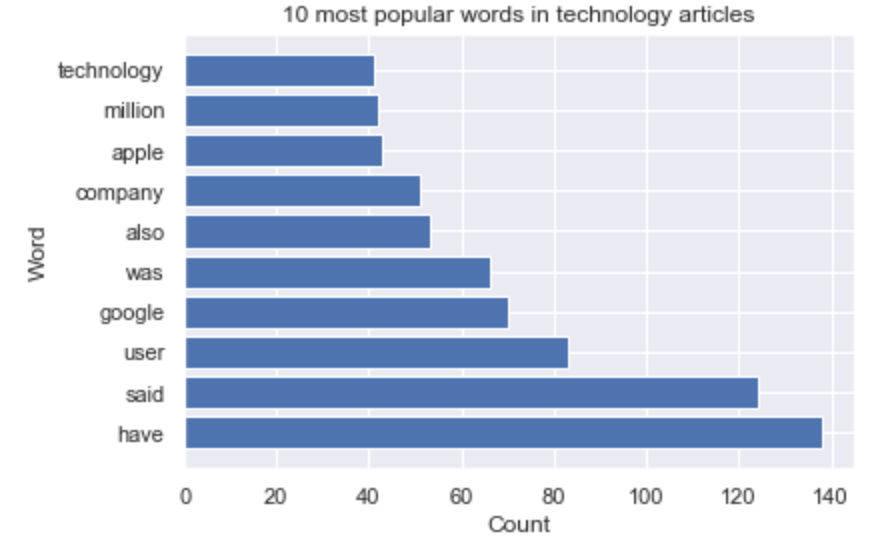
\includegraphics[width=\textwidth]{images/analiza/technology.png}
     \end{subfigure}
        \caption{Najpopularniejsze wyrazy w każdej z analizowanych kategorii}
        \label{fig:10_most_popular_words}
\end{figure}

\newpage
\newpage
Kolejnym analizowanym aspektem są bi-gramy, czyli częstotliwość występowania dwóch słów obok siebie. Na podstawie zebranych danych wygląda to następująco:

\begin{figure}[H]
     \centering
     \begin{subfigure}[b]{0.7\textwidth}
         \centering
         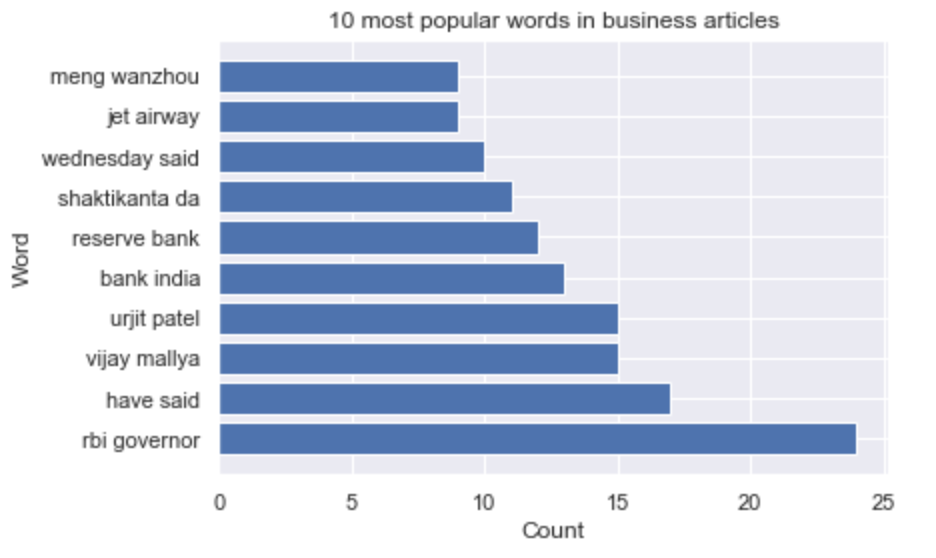
\includegraphics[width=\textwidth]{images/analiza/business_bigram.png}
     \end{subfigure}
     \hfill
     \begin{subfigure}[b]{0.7\textwidth}
         \centering
         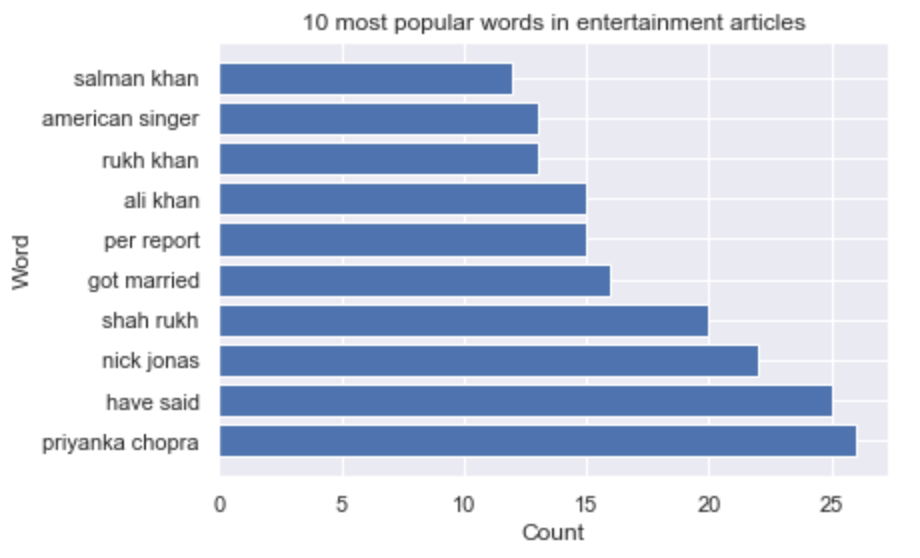
\includegraphics[width=\textwidth]{images/analiza/entertainment_bigram.png}
     \end{subfigure}
     \hfill
     \begin{subfigure}[b]{0.7\textwidth}
         \centering
         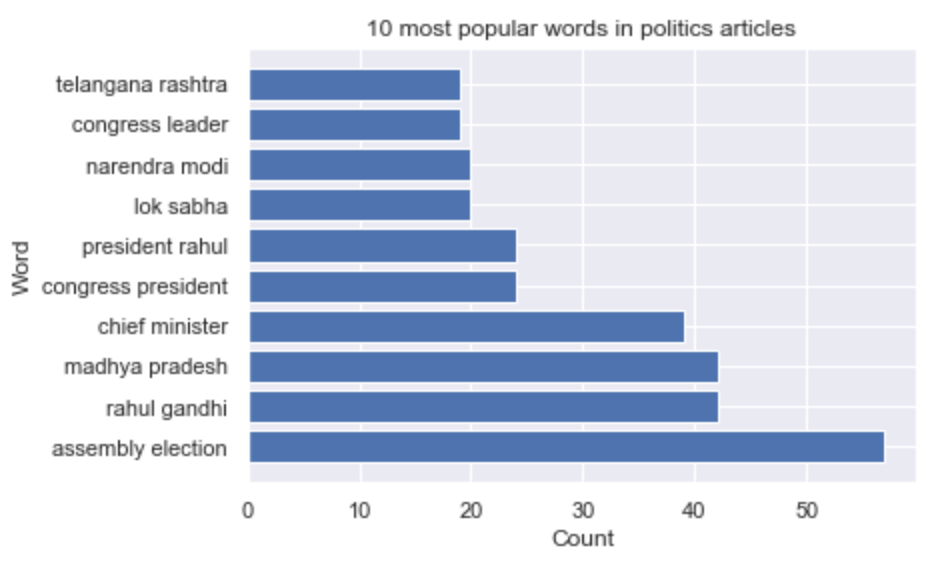
\includegraphics[width=\textwidth]{images/analiza/politics_bigram.png}
     \end{subfigure}
\end{figure}
\begin{figure}[H]\ContinuedFloat
     \begin{subfigure}[b]{0.7\textwidth}
         \centering
         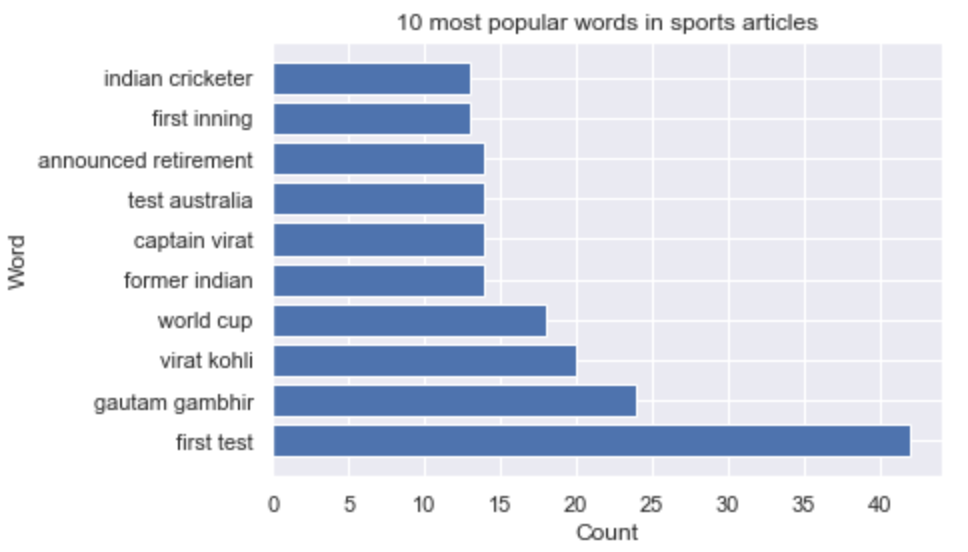
\includegraphics[width=\textwidth]{images/analiza/sports_bigram.png}
     \end{subfigure}
     \hfill
     \begin{subfigure}[b]{0.7\textwidth}
         \centering
         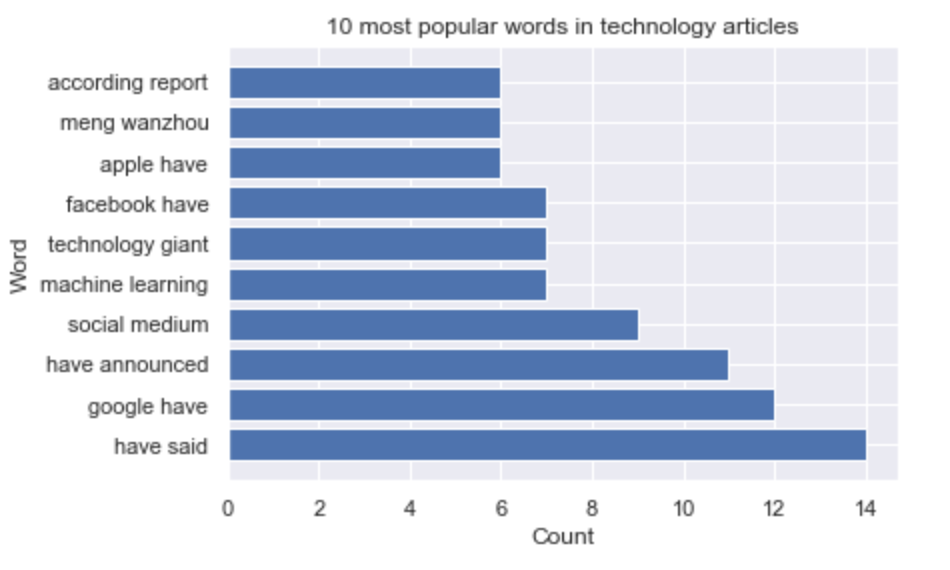
\includegraphics[width=\textwidth]{images/analiza/technology_bigram.png}
     \end{subfigure}
        \caption{Najpopularniejsze 2-gramy w każdej z analizowanych kategorii}
        \label{fig:10_most_popular_ngrams}
\end{figure}

Pojawiło się tutaj pewne zakłócenie - z racji, że dane pochodzą z jednego źródła pojawiło się kilka imion i nazwisk osób oraz nazw własnych. Jednak jest też kilka ciekawych pozycji takich jak 'have announced' w kategorii artykułów technologicznych, czy 'assembly election' dotyczących polityki. Prawdopodobnie przy zaczerpnięciu danych z większej ilości źródeł wyniki byłyby dużo bardziej satysfakcjonujące.

\newpage
\section{Test klasyfikatorów}

W celu wybrania najlepszych klasyfikatorów wybrałem dwa modele przetworzenia danych: bag of words oraz term frequency - inverse document frequency. Dane zostały podzielone na zbiór treningowy oraz testowy w stosunku 8:2. Wyniki testu znajdują się na poniższym wykresie. Przedstawiają one uzyskaną skutecznośc algorytmu, czyli jaka część danych ze zbioru testowego została poprawnie sklasyfikowana.

\begin{figure}[H]
     \centering
     \begin{subfigure}[b]{0.8\textwidth}
         \centering
         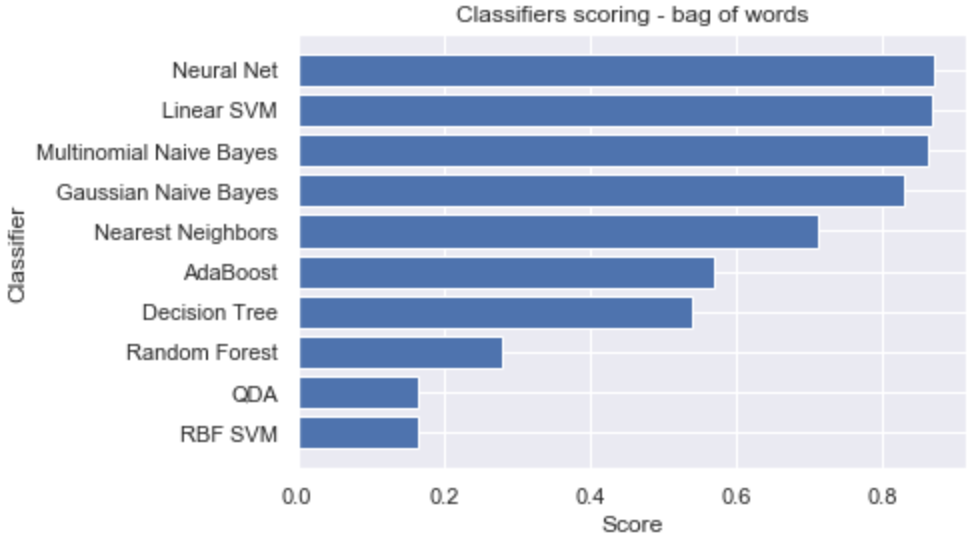
\includegraphics[width=\textwidth]{images/analiza/classifiers_bag.png}
     \end{subfigure}
     \hfill
     \begin{subfigure}[b]{0.8\textwidth}
         \centering
         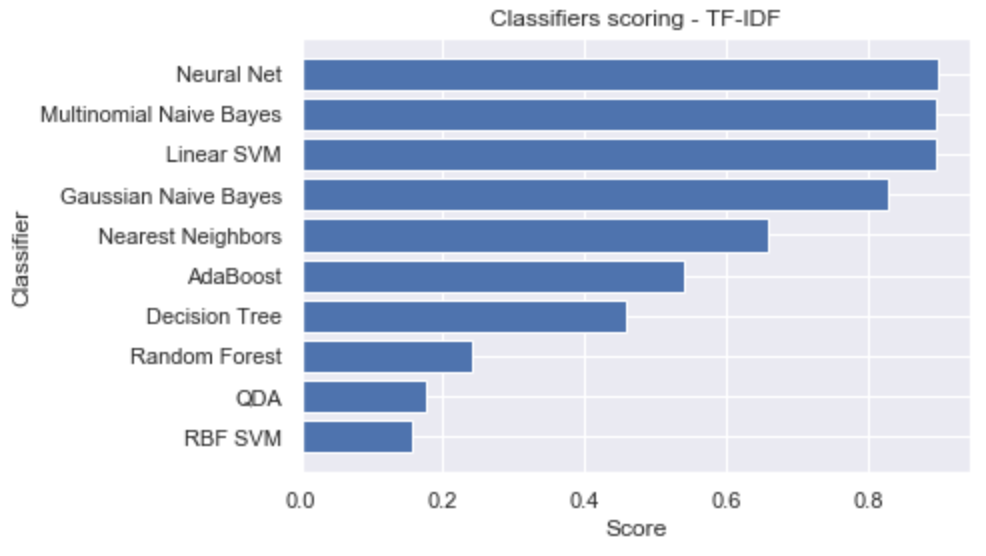
\includegraphics[width=\textwidth]{images/analiza/classifiers_tfidf.png}
     \end{subfigure}
        \caption{Skuteczność różnych klasyfikatorów}
        \label{fig:classifiers_test}
\end{figure}

Z tego badania można wywnioskować, że użyty model danych (bag of words/TF-IDF) nie miał znaczącego wpływu na skuteczność algorytmów uczenia nadzorowanego. W obu przypadkach obiecujące wyniki uzyskały trzy algorytmy:
\begin{enumerate}
    \item Sieć neuronowa.
    \item Liniowa maszyna wektorów nośnych.
    \item Naiwny klasyfikator bayesowski (w dwóch wariacjach).
\end{enumerate}

\section{Klasteryzacja}

W ramach przeprowadzanych doświadczeń, postanowiłem również sprawdzić jak zebrane dane będą podatne na uczenie nienadzorowane. Badania rozpocząłem od użycia algorytmu k-średnich (ang. k-means) na przetworzonych danych i próbie podzielenia ich na klastry.

Do walidacji rezultatów wykorzystałem kategorie przypisane do danych. Dla idealnie działającego algorytmu klasteryzacji jedna kategoria powinna występować tylko w jednym klastrze. Początkowo wykonałem dzielenie danych na dwa klastry - przeprowadziłem ten zabieg dwa razy (raz dla danych w formie Bag of Words, a raz jako TF-IDF).

    \begin{figure}[H]
    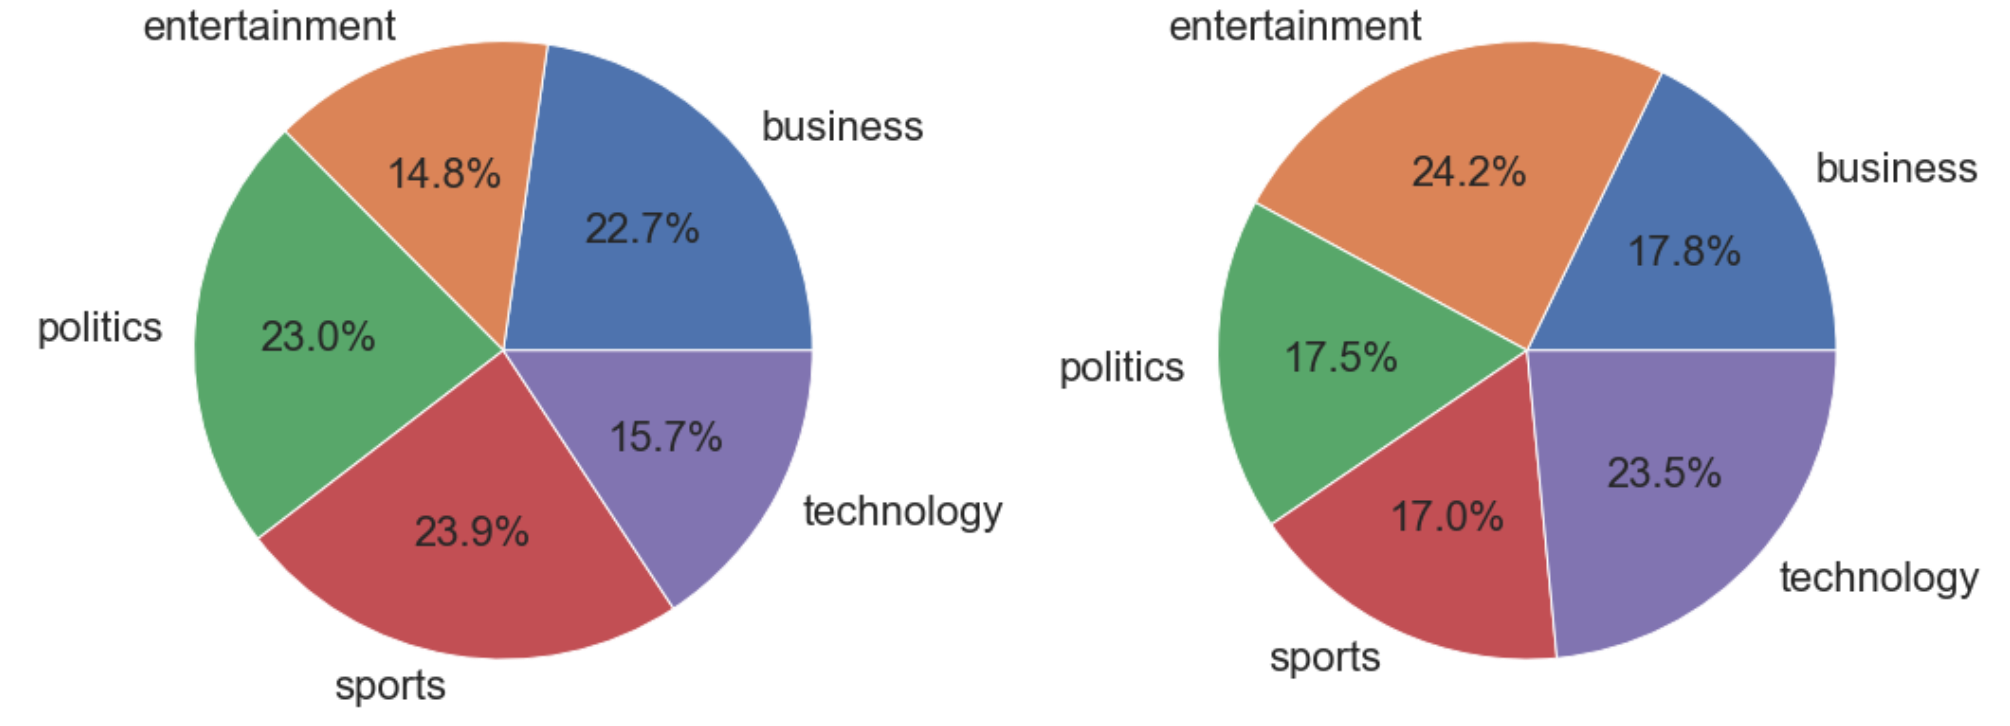
\includegraphics[width=\textwidth]{images/analiza/klast_bow.png}
    \centering
    \caption{Dwa klastry uzyskane z modelu Bag of Words}
    \label{fig:cls1}
    \end{figure} 
    
    \begin{figure}[H]
    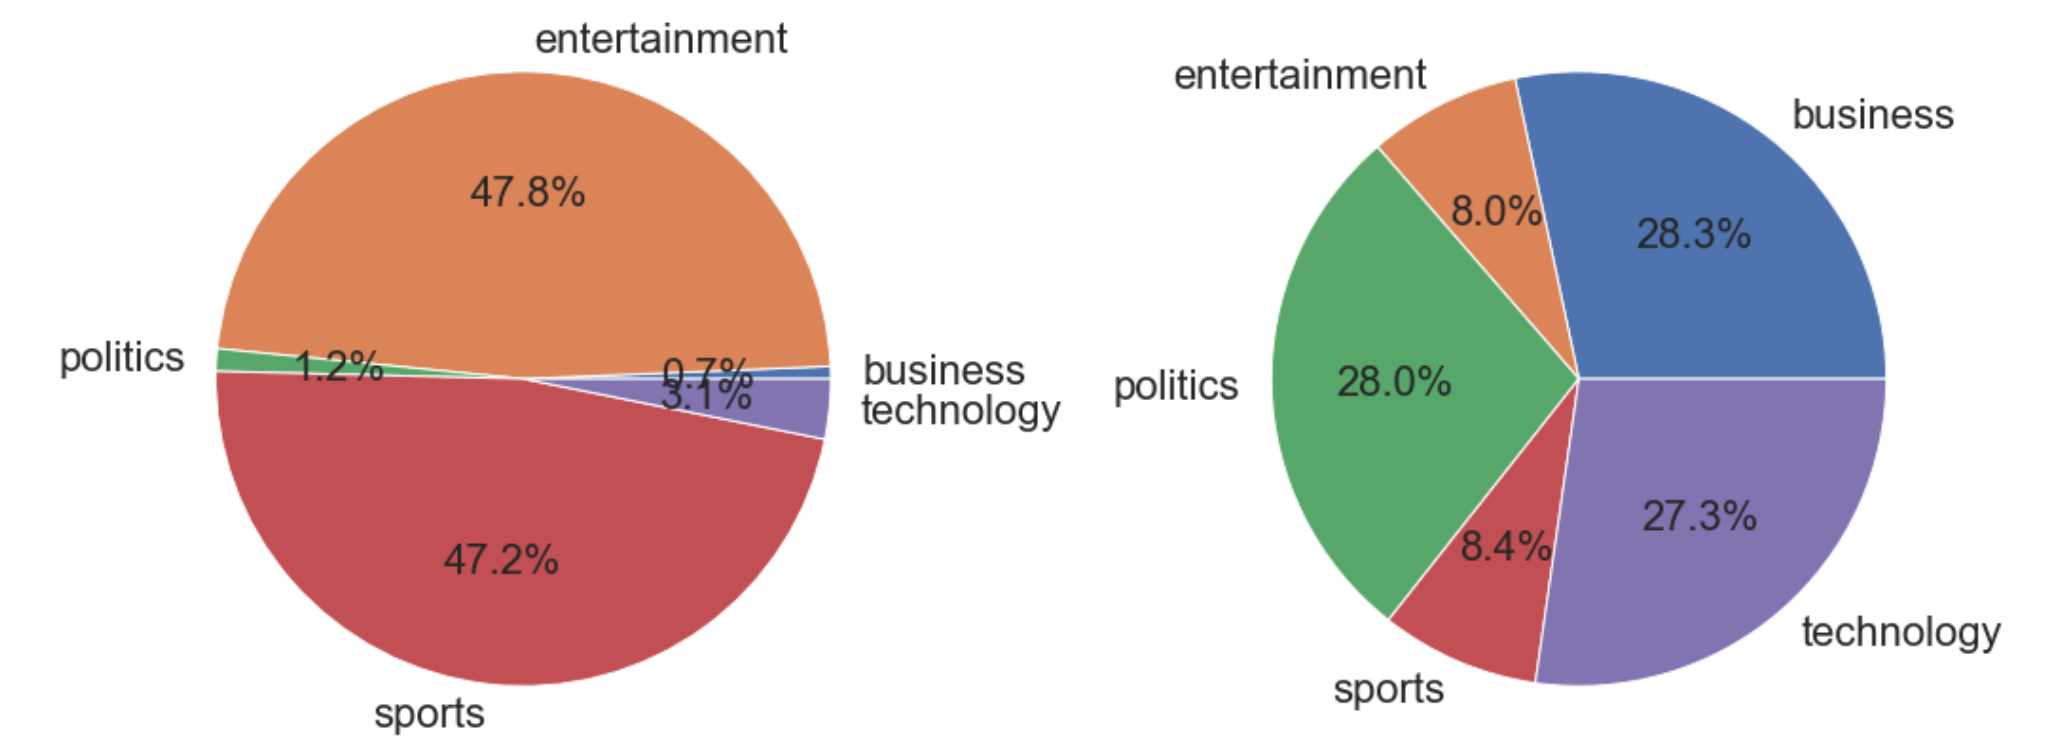
\includegraphics[width=\textwidth]{images/analiza/klast_tfidf.png}
    \centering
    \caption{2 klastry uzyskane z modelu TF-IDF}
        \label{fig:cls2}
    \end{figure} 

Na rysunku \ref{fig:cls2} widać wyraźne oddzielenie kategorii sport i rozrywka od reszty danych. Wskazuje to na fakt, że model TF-IDF wykazuje większą podatność na klasteryzację niż klasyczny Bag of Words. Dalsze próby będą kontynuowane bazując jedynie na danych TF-IDF.

W kolejnej próbie dane zostały podzielone na 5 klastrów, czyli tyle ile jest kategorii, którymi dane są oznaczone. Wizualizacja przedstawiona jest w odwrotnej formie - każdy wykres reprezentuje jedną kategorię i zawiera numery klastrów do których trafiły artykuły do niej należące.

\begin{figure}[H]
     \centering
     \begin{subfigure}[b]{0.38\textwidth}
         \centering
         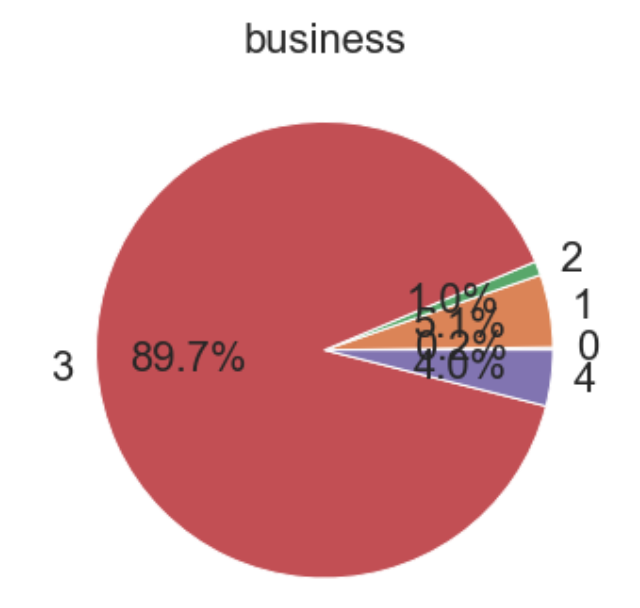
\includegraphics[width=\textwidth]{images/analiza/c_b.png}
     \end{subfigure}
     \hfill
     \begin{subfigure}[b]{0.34\textwidth}
         \centering
         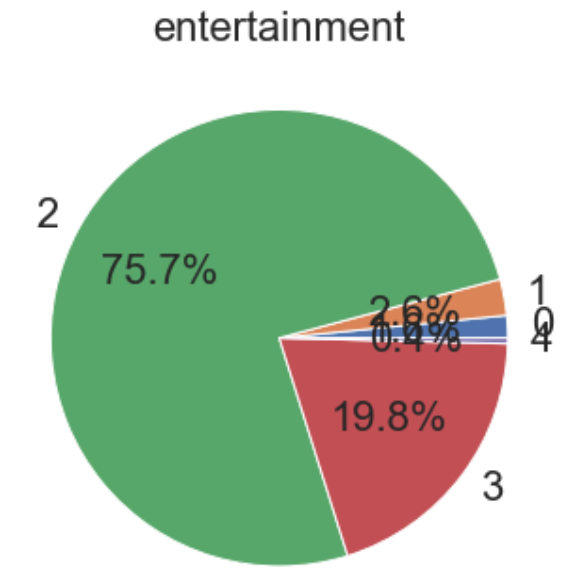
\includegraphics[width=\textwidth]{images/analiza/c_e.png}
     \end{subfigure}
     \hfill
     \begin{subfigure}[b]{0.38\textwidth}
         \centering
         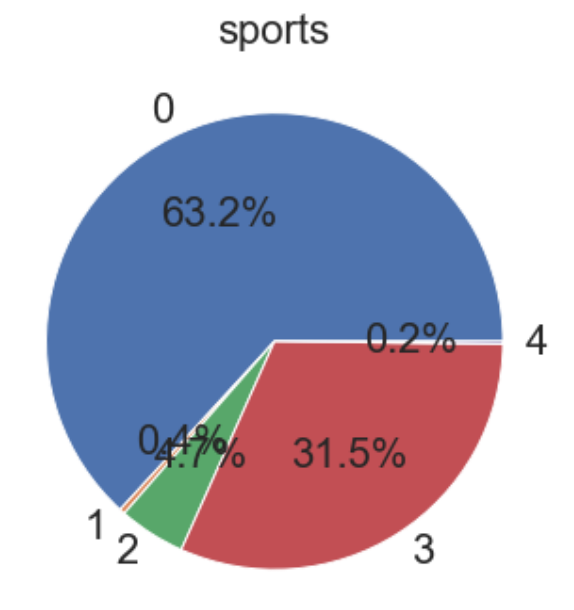
\includegraphics[width=\textwidth]{images/analiza/c_s.png}
     \end{subfigure}
     \hfill
     \begin{subfigure}[b]{0.38\textwidth}
         \centering
         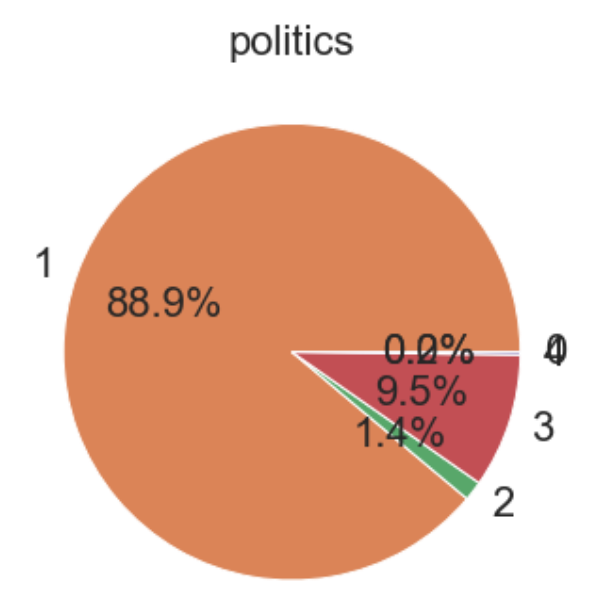
\includegraphics[width=\textwidth]{images/analiza/c_p.png}
     \end{subfigure}
     \hfill
     \begin{subfigure}[b]{0.38\textwidth}
         \centering
         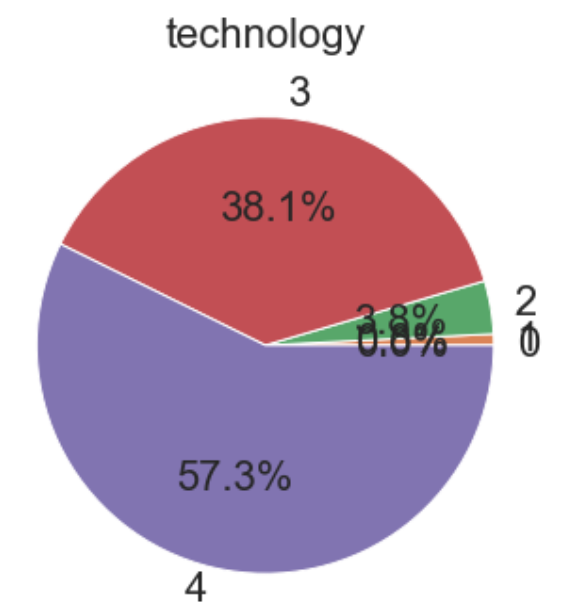
\includegraphics[width=\textwidth]{images/analiza/c_t.png}
     \end{subfigure}
        \caption{Rezultat podzielenia danych na 5 klastrów.}
        \label{fig:classifiers_test}
\end{figure}

Wyniki są zadowalające - artykuły rozrywkowe, technologiczne, polityczne i sportowe znalazły się w przeważającej mierze we własnych klastrach. Jedynie w klastrze 3, który zawiera w większości artykuły biznesowe znalazło się sporo artykułów o innej tematyce.


\chapter{Implementacja systemu kategoryzacji}
\label{cha:implementacja}

System kategoryzacji jest kompletną aplikacją, która oferuje gromadzenie danych, przetwarzanie ich, wyliczanie rezultatów, a także interakcję z użytkownikiem. Modelowo taki system powinien zawierać trzy elementy:
\begin{enumerate}
    \item Warstwa persystencji danych.
    
    Element systemu, który ma za zadanie trwałe przechowywanie danych. Zwykle jego rolę pełni baza relacyjna. Możliwe jest jednak wykorzystanie innych systemów takich jak bazy nierelacyjne (NoSQL). Głównym założeniem tego elementu jest zachowywanie stanu aplikacji nawet jeśli zostanie ona zamknięta.
    
    \item Warstwa logiki aplikacji.
    
    Część odpowiadająca za przetwarzanie zapytań użytkownika, komunikację z bazą danych oraz przetwarzanie danych. Zazwyczaj modeluje ona pewne procesy biznesowe.
    
    \item Warstwa prezentacji.
    
    Element odpowiedzialny bezpośrednio za interakcję z użytkownikiem. Przekazuje on żądania użytkownika do warstwy logiki aplikacji oraz prezentuje odpowiedzi w czytelnej dla człowieka formie. Pełni ona bardzo ważną rolę w kwestii odbioru aplikacji przez użytkownika.
\end{enumerate}

\section{Warstwa persystencji danych}

Jako warstwę przechowywującą dane aplikacji użyłem produktu firmy Amazon - DynamoDB. Jest to baza nierelacyjna charakteryzująca się niskim kosztem zapisu i odczytu danych. Została ona obszernie opisana w rozdziale \ref{cha:wprowadzenieTechnologiczne}.

W procesie implementacji aplikacji używałem DynamoDB w dwóch formach:

\begin{enumerate}
    \item Zdalnie poprzez platformę Amazon Web Service.
    
    AWS jest jedynym miejscem w którym mamy możliwość ustawienia DynamoDB w wersji produkcyjnej. Najważniejszym parametrem jej konfiguracji jest region, czy miejsce gdzie nasza baza będzie się fizycznie znajdowała. Najkorzystniejszym wyborem jest ten sam region w którym działa aplikacja - wtedy opóźnienie w przesyłaniu danych będzie najmniejsze.
    
    \item Na lokalnym środowisku.
    
    Amazon udostępnia nam trzy sposoby na uruchomienie DynamoDB na środowisku lokalnym:
    
    \begin{enumerate}
        \item Poprzez plik .jar
        \item Używając narzędzia budowania aplikacji - Apache Maven
        \item Poprzez obraz Dockera
    \end{enumerate}
    
    Z powodu dobrej znajomości Dockera zdecydowałem się na trzeci sposób. Obraz znajduje się w oficjalnym rejestrze \footnote{https://hub.docker.com/r/amazon/dynamodb-local/} i jesteśmy w stanie go pobrać i uruchomić przy użyciu jednej komendy (pod warunkiem, że mamy zainstalowanego Dockera):
    
    \begin{verbatim}
        docker run -p 8000:8000 amazon/dynamodb-local
    \end{verbatim}
    
    Po wykonaniu tej operacji lokalna instancja DynamoDB jest dostępna na porcie 8000. Z tak skonfigurowanym środowiskiem jesteśmy w stanie komunikować się na dwa sposoby:
    
    \begin{enumerate}
        \item AWS CLI
        
        Jest to narzędzie konsolowe do obsługi usług AWS. Z jego pomocą jesteśmy w stanie tworzyć oraz zarządzać serwisami umieszczonymi w chmurze Amazona. W DymanoDB nową tabelę możemy stworzyć za pomocą komendy:
        
        \begin{verbatim}
aws dynamodb create-table \
    --table-name User \
    --attribute-definitions \
        AttributeName=Id,AttributeType=S \
        AttributeName=Name,AttributeType=S \
    --key-schema 
        AttributeName=Id,KeyType=HASH \
        AttributeName=Name,KeyType=RANGE \
    --provisioned-throughput ReadCapacityUnits=1,WriteCapacityUnits=1
    --endpoint-url http://192.168.99.100:8000
        \end{verbatim}
        
        Należy zauważyć, że parametr endpoint-url wskazuje na lokalną instancję DynamoDB uruchomioną w kontenerze Dockera. Gdyby nie został on podany wtedy AWS CLI wymaga uwierzytelnienia się w usłudze AWS i próbowałby utworzyć zasoby w chmurze.
        
        \item AWS SDK
        
        Amazon zapewnia nam obszerne SDK do wielu języków programowania. Pozwala to na wygodną integrację z usługami AWS z tworzonymi aplikacjami. W systemie tworzonym w ramach tej pracy korzystałem z języka Python, do którego AWS SDK znajduje się w ramach pakietu boto3. Przykład tworzenia analogicznej tabeli poprzez AWS SDK:
        
        \begin{verbatim}
boto3.resource('dynamodb', endpoint_url='http://localhost:8000')\
.create_table(
    TableName='Users',
    KeySchema=[
        {
            'AttributeName': 'label',
            'KeyType': 'HASH'
        },
        {
            'AttributeName': 'content',
            'KeyType': 'RANGE'
        }
    ],
    AttributeDefinitions=[
        {
            'AttributeName': 'label',
            'AttributeType': 'S'
        },
        {
            'AttributeName': 'content',
            'AttributeType': 'S'
        }
    ],
    ProvisionedThroughput={
        'ReadCapacityUnits': 1,
        'WriteCapacityUnits': 1
    }
)
        \end{verbatim}
    \end{enumerate}
    
\end{enumerate}

\subsection{Struktura danych}

Charakterystyka rozproszonych nierelacyjnych baz danych wymaga od programisty specjalnego podejścia do projektowania struktury w jakiej dane będą przechowywane. W bazach relacyjnych dąży się do jak najlepszej normalizacji i braku duplikacji. Podczas, gdy używamy DynamoDB każda tabela może być rozproszona na wiele partycji, przez co ilość danych nie stanowi ograniczenia. Również koszt ich przechowywania jest niski, przez co warto duplikować dane, jeśli może to mieć wpływ na szybkość działania systemu.

W podstawowym modelu danych przechowywanych w ramach systemu klasyfikacji skupiłem się na prostej strukturze zwierającej trzy atrybuty:

\begin{enumerate}
    \item Label - kategoria która opisuje daną próbkę
    
    \item Source - źródło z którego próbka pochodzi
    
    \item Content - zawartość próbki
\end{enumerate}

Projektowanie tabel w DynamoDB najlepiej zacząć od ustalenia jakie kwerendy będziemy chcieli na nich wykonywać. W przypadku powyższych danych ustaliłem dwie opcje:

\begin{enumerate}
    \item Pobieranie danych według atrybutu 'Label'
    
    \item Pobieranie danych według atrybutu 'Source'
\end{enumerate}

Dodatkowym założeniem, które przyjąłem był brak duplikatów w poszczególnych tabelach. Uczenie algorytmów zduplikowanymi próbkami zaburzałoby cały proces i mogło by prowadzić do błędnych wyników. Z tego powodu zdecydowałem się zapewnić unikalność danych na poziomie warstwy persystencji danych.

Biorąc pod uwagę powyższe wymagania zdecydowałem się na poniższy schemat:

\begin{figure}[H]
    \centering
    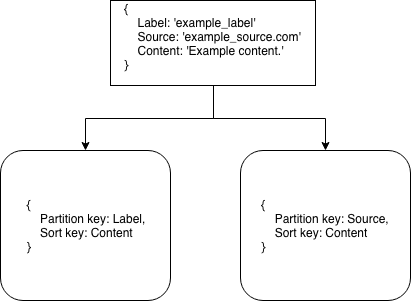
\includegraphics[width=10cm]{data_structure.png}
    \caption{Struktura danych}
\end{figure}

Pierwszą ważną cechą jest zduplikowanie danych w dwóch tabelach - na każdej bedzie wykonywana inna kwerenda. Tabela 'content\_by\_label' posłuży do odczytania danych po atrybucie 'Label', natomiast gdy chcemy pobrać wszystkie dane pochodzące z jednego źródła, wtedy użyjemy tabeli 'content\_by\_source'.

Unikalność danych zapewniło nam użycie Primary Key z dwoma atrybutami. Primary Key składa się z dwóch części:

- Partition key - atrybut, którego hash określi na której partycji znajdzie się dany rekord

- Sort key - atrybut według którego dane będą posortowane w obrebie partycji

Primary key musi być zawsze unikalny. Z tego powodu zastosowanie par ('Label', 'Content') oraz ('Source', 'Content') pozwoliło mi zapewnić unikalność danych w obrębie każdej z tabel.

\begin{figure}[H]
    \centering
    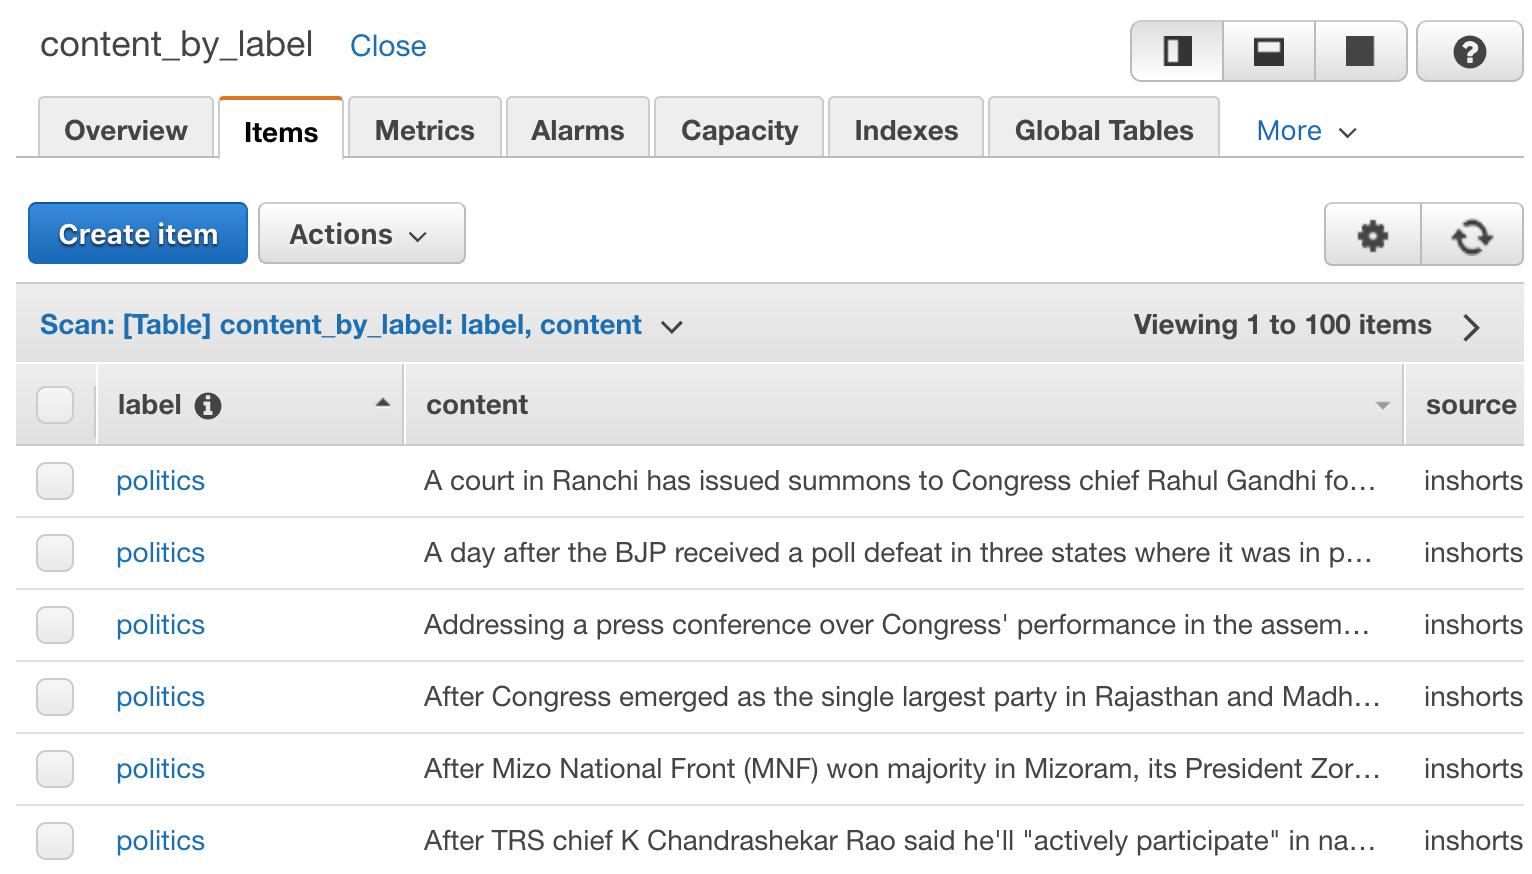
\includegraphics[width=10cm]{dynamo_by_label.png}
    \caption{Fragment tabeli content\_by\_label widocznej z poziomu konsoli AWS}
\end{figure}

\begin{figure}[H]
    \centering
    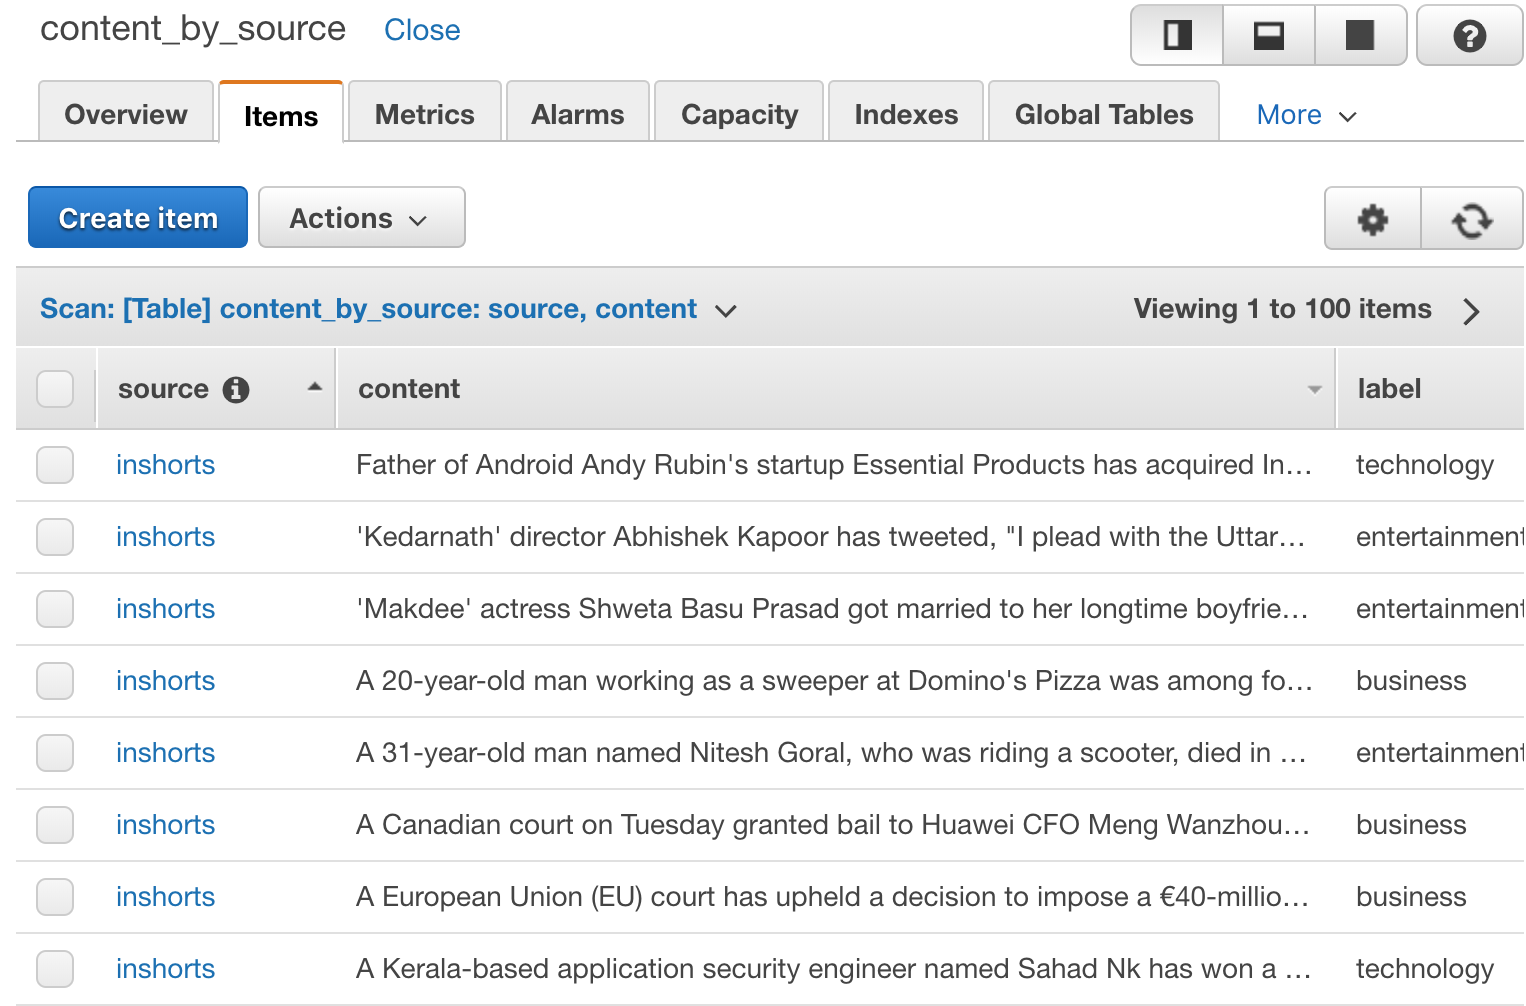
\includegraphics[width=10cm]{dynamo_by_source.png}
    \caption{Fragment tabeli content\_by\_source widocznej z poziomu konsoli AWS}
\end{figure}

\newpage
\section{Warstwa logiki aplikacji}

Elementem centralnym systemu kategoryzacji jest aplikacja komunikująca się z bazą danych używając AWS SDK oraz z warstwą prezentacji danych używając protokołu HTTP. Została ona napisana w języku Python przy użyciu frameworku Flask. Aplikacja jest napisana z wykorzystaniem paradygmatu programowania obiektowego oraz ma budowę komponentową.

\subsection{Python}

Wybór języka programowania zawsze jest pewnym wyzwaniem dla architektów systemu. W tej pracy zdecydowałem się użyć języka Python z następujących powodów:

\begin{enumerate}
    \item Dynamiczne typowanie
    
    Ta cecha języka pozwala nam na bardziej produktywne pisanie pisanie kodu aplikacji. Dynamiczne typowanie zazwyczaj wymaga mniej kodu do wykonania poszczególnych operacji niż statycznie typowane języki. Niestety często skutkuje ona większą podatnością na błędy podczas działania aplikacji.
    
    \item Narzędzia do uczenia maszynowego oraz przetwarzania danych
    
    Popularność języka Python wśród profesjonalistów zajmujących się uczeniem maszynowym oraz analizą danych przyczyniła się do szybkiego rozwoju solidnych narzędzi przystosowanych do tych celów. Pakiety takie jak pandas \footnote{https://pandas.pydata.org/}, tensorflow \footnote{https://www.tensorflow.org}, czy scikit-learn \footnote{https://scikit-learn.org/stable/} znacznie ułatwiają pracę z danymi oraz przyczyniają się do ciągłego rozwoju języka w tym kierunku.
    
    \item Rosnąca popularność
    
    Według raportów portalu Stack Overflow (Rys. \ref{fig:python_popularity}) od roku 2012 ilość pytań zadawanych dla języka Python ma stale tendencję rosnącą, a w ostatnich miesiącach była większa niż dwa kolejne najpopularniejsze języki - Java oraz Javascript. To oznacza stale rosnącą społeczność skupioną wokół tego języka, co znacznie usprawnia proces rozwoju technologii.
    
    \begin{figure}[H]
        \centering
        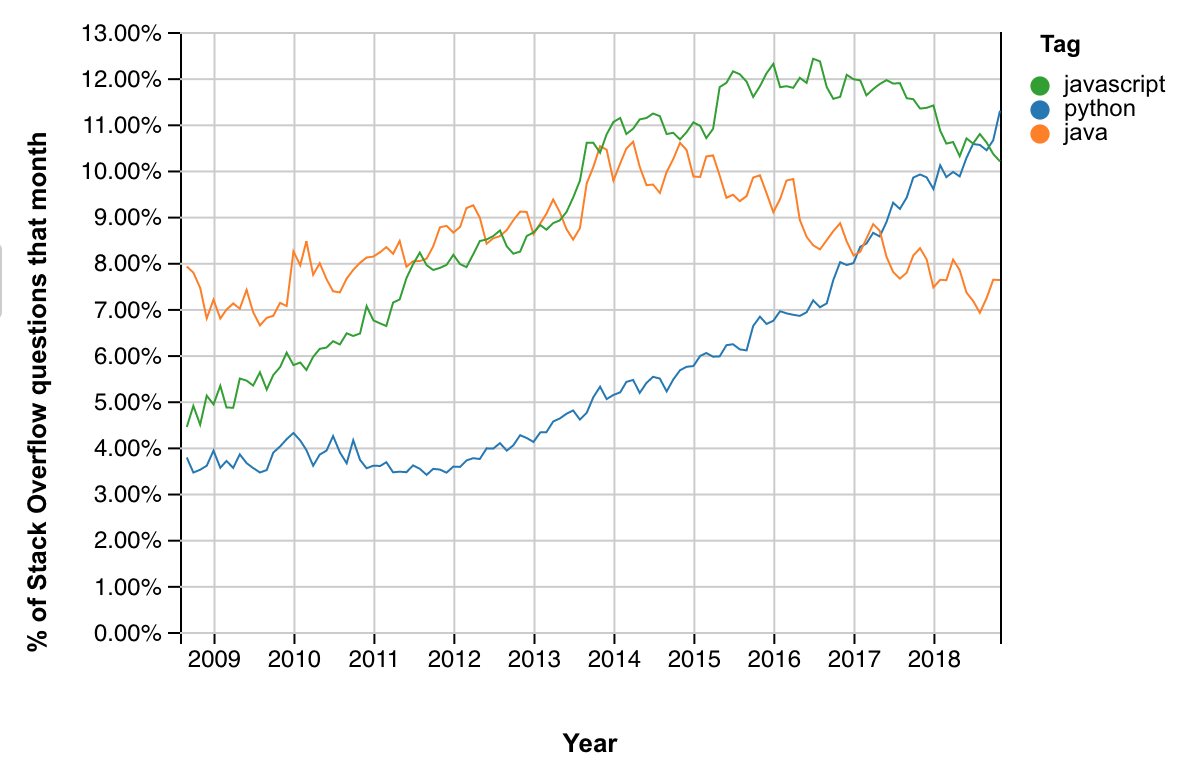
\includegraphics[width=10cm]{python_popularity.png}
        \caption{Popularność pytań o dany język programowania według tagów na Stack Overflow. Źródło: https://insights.stackoverflow.com/trends}
        \label{fig:python_popularity}
    \end{figure}
    
\end{enumerate}

\subsection{Flask framework}

W przeniesieniu logiki na aplikację wykorzystałem projekt Flask \footnote{http://flask.pocoo.org/}. Jest on określany przez autorów jako "microframework" do rozwijania aplikacji webowych. Charakteryzuj go niski próg wejścia - napisanie aplikacji typu "Hello world" to zaledwie 5 linii kodu:

\begin{lstlisting}[language=Python]
from flask import Flask
app = Flask(__name__)

@app.route("/greeting")
def hello():
    return "Hello Flask!"
\end{lstlisting}

W systemie kategoryzacji Flask zapewnił wszystkie funkcjonalności w ramach serwera HTTP, dzięki czemu po jego wdrożeniu będą one dostępne z każdego urządzenia podłączonego do internetu.

\subsection{Architektura}

Z aplikacji można wydzielić dwa główne moduły:
\begin{enumerate}
    \item Moduł danych.
    
    Moduł odpowiadający za gromadzenie, zapis, odczyt oraz migrację danych. Jego podstawowym zadaniem jest pobieranie danych z internetu, przetworzeniu ich do formy możliwej do zapisu (również parsowanie HTML) oraz zapis do bazy danych.
    
    \item Moduł analizy i klasyfikacji.
    
    Pobiera on przygotowane już dane z bazy danych i wykorzystuje je do analizy. Ma również możliwość pobrania wejścia od użytkownika i wykorzystania algorytmów uczenia maszynowego do klasyfikacji wejściowego tekstu.
\end{enumerate}

Każdy moduł jest stworzony zgodnie z paradygmatem programowania obiektowego. Jest on podzielony na klasy, które zostały zaprojektowane zgodnie z zasadami SOLID \footnote{https://pl.wikipedia.org/wiki/SOLID_(programowanie_obiektowe)}

\subsection{Komunikacja z użyciem protokołu HTTP}

Z aplikacją można się komunikować używając protokołu HTTP. Poniżej podane są przykładowe zapytania, których możemy użyć. Pierwsza część określa metodę zapytania, a druga adres URL oraz parametry.

Pobranie danych ze wskazanego źródła:
\begin{verbatim}
    GET {{host}}/data/download?source={{source}}&count={{count}}
    
    {{host}} - adres pod jakim działa aplikacja
    {{source}} - źródło z jakiego chcemy pobrać dane (nazwa API)
    {{count}} - ilość danych jaką chcemy pobrać
\end{verbatim}

Pobranie danych ze wskazanego źródła oraz zmigrowanie ich do bazy danych:
\begin{verbatim}
    POST {{host}}/data/migration?source={{source}}&count={{count}}
\end{verbatim}

Kategoryzacja danych wejściowych na podstawie zmigrowanych danych:
\begin{verbatim}
    GET {{host}}/classify?size={{dataset_size}}&q={{input}}&model={{model}}
    
    {{dataset_size}} - rozmiar zestawu uczącego jaki chcemy użyć
    {{model}} - algorytm uczenia maszynowego za pomocą którego chcemy 
    wykonać klasyfikację
    {{input}} - dane wejściowe dla których wykonujemy kategoryzacją
\end{verbatim}

\newpage
\section{Warstwa prezentacji}

Interfejs użytkownika jest nieodłącznym elementem każdego kompletnego systemu komputerowego. Forma przedstawienia funkcjonalności naszego systemu jest bardzo ważnym aspektem, którego zaniedbanie może zniechęcić użytkowników do korzystania z naszego rozwiązania. Obecnie dużą popularnością cieszą się aplikacje webowe. Są one zbudowane na podstawie dobrze znanych technologii, oraz co najważniejsze - można je otworzyć na wszystkich urządzeniach z zainstalowaną przeglądarką internetową. Spowodowały one częściowe wyparcie technologii desktopowych, które wymagały instalacji oprogramowania na urządzeniu klienta przed jego otworzeniem. Obserwuje się również trend porzucania aplikacji mobilnych na rzecz webowych przystosowanych do telefonów i tabletów.

Z racji popularności technologii HTML, CSS oraz Javascript przeglądarki internetowe stają się coraz bardziej rozbudowanymi narzędziami. Wszystkie popularne przeglądarki udostępniają narzędzia do tworzenia dodatków do nich, a niektóre (np. Google Chrome) oferują możliwość tworzenia aplikacji desktopowych opartych na przeglądarce. Istnieją również projekty jak Electron \footnote{https://electronjs.org/}, które umożliwiają bezpośrednie przekonwertowanie kodu strony internetowej na aplikację uruchamianą bez udziału przeglądarki.

\subsection{Wybór technologii}

Jako warstwę prezentacji do budowanego systemu zdecydowałem się użyć dodatku do przeglądarki Google Chrome. W przypadku systemu kategoryzacji tekstu zaważyły o tym następujące czynniki:
\begin{enumerate}
    \item Możliwość interakcji ze wszystkimi stronami internetowymi.
    
    Internet jest bardzo bogatym źródłem danych w formie tekstu. Poprzez dodatek do przeglądarki użytkownik będzie miał możliwość interakcji z danymi zawartymi w serwisach internetowych i ich analizę i klasyfikację z wykorzystaniem serwisu rozwijanego w ramach tej pracy.
    
    \item Wykorzystanie technologii webowych.
    
    Dodatki do przeglądarek są implementowane w językach używanych do budowy aplikacji webowych. Oznacza to niski próg wejścia - każdy kto miał styczność z językiem Javascript powinien poradzić sobie z ich tworzeniem. Dodatkowo przeniesienie kodu takiej aplikacji do przeglądarki lub na desktop nie będzie wymagało przepisania jej w całości.
\end{enumerate}

Platforma na którą planowałem wdrożyć rozwiązanie to Google Chrome. Według danych NetMarketShare \footnote{https://netmarketshare.com/browser-market-share.aspx} z roku 2018 jest to obecnie najpopularniejsza przeglądarka internetowa:

\begin{figure}[H]
    \centering
    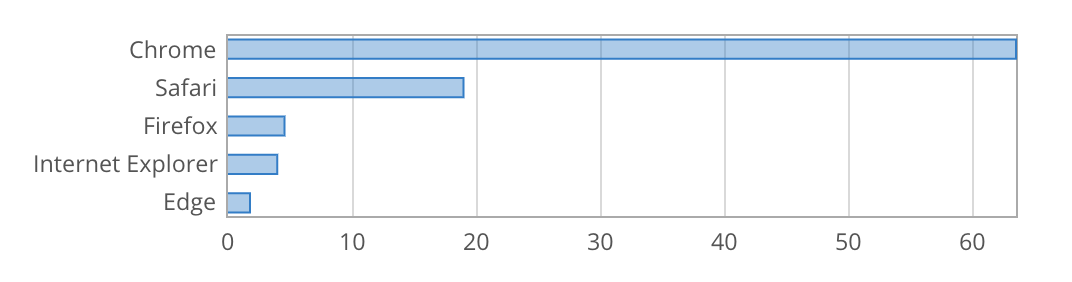
\includegraphics[width=10cm]{browser_market_share.png}
    \caption{Udział przeglądarek w rynku wyrażony w punktach procentowych według NetMarketShare }
\end{figure}

\subsection{Implementacja}

Sercem kodu zawierającego dodatek do przeglądari Google Chrome jest plik manifest.json - dla tej pracy wygląda on tak jak poniżej:

\begin{lstlisting}[language=json]
{
  "manifest_version": 2,
  "name": "Text Recognizer",
  "description": "Extension for recognizing text.",
  "version": "0.1",
  "permissions": [
    "tabs",
    "contextMenus",
    "<all_urls>",
    "storage"
  ],
  "browser_action": {
    "default_popup": "popup.html",
    "default_title": "Text Recognizer"
  },
  "content_scripts": [
    {
      "matches": [
        "<all_urls>"
      ],
      "js": [
        "selection.js"
      ],
      "run_at": "document_start",
      "all_frames": true
    }
  ],
  "background": {
    "scripts": ["background.js"]
  },
  "options_ui": {
    "page": "options.html",
    "open_in_tab": false
  }
}
\end{lstlisting}

Poza definicjami wyświetlanych tytułów oraz wersjonowania zawiera on najważniejsze informacje o pozwoleniach na akcje oraz dostęp do poszczególnych elementów przeglądarki. Pozostałe sekcje obejmują informacje o strukturze dodatku: 

\begin{enumerate}
    \item Browser action
    
    Definiuje tytuł oraz ścieżkę do elementu typu pop-up, który pojawia się w momencie kliknięcia na ikonę dodatku.
    
    \begin{figure}[H]
    \centering
    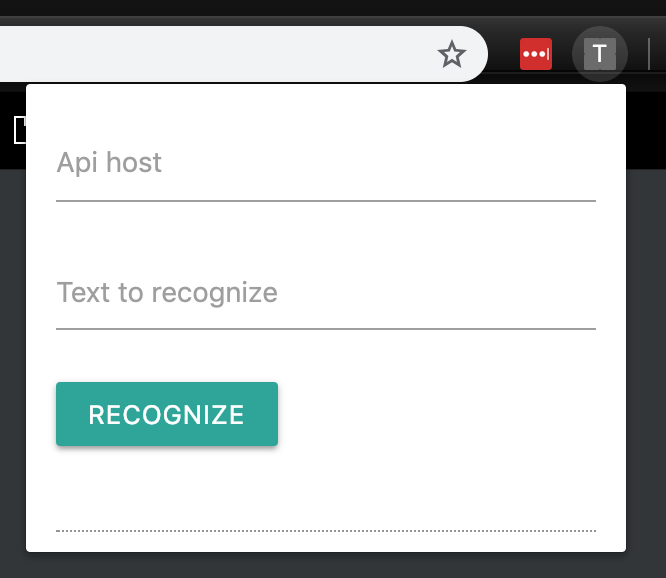
\includegraphics[width=10cm]{images/implementacja/popup.png}
    \caption{Popup}
    \end{figure}
    
    \item Content scripts
    
    Problem związanym ze wspomnianym wcześniej elementem zdefiniowanym jako browser action jest posiadanie osobnego elementu DOM (Document Object Model\footnote{https://www.w3.org/TR/DOM-Level-2-HTML/}). Poprzez sam popup nie mamy możliwości jakiejkolwiek interakcji z obecnie otworzoną stroną internetową. Rozwiązaniem jest użycie content script, który jest uruchamiany w kontekście strony. Ma on możliwość interakcji z modelem DOM oraz komunikacji z elementem popup poprzez system wiadomości. W mojej aplikacji content script służy do przesłania zaznaczonego tekstu do elementu popup, jeśli dostanie takie żądanie w wiadomości. Jego kod wygląda tak jak poniżej:
    
    \begin{lstlisting}[language=javascript]
    chrome.extension.onMessage.addListener((request, sender, sendResponse) => {
    if (request.method == "getSelection")
        sendResponse({data: window.getSelection().toString()});
    else
        sendResponse({data: ''});
    });
    \end{lstlisting}
    
    \item Background
    
    Skrypty zdefiniowane w sekcji background działają w tle strony niezależnie od jej zawartości. Wykorzystuję go do ustawienia nowego elementu w menu kontekstowym, ustawienia funkcji 'onclick' oraz przekazanie do niej obecnie zaznaczonego tekstu.
    
    \begin{figure}[H]
    \centering
    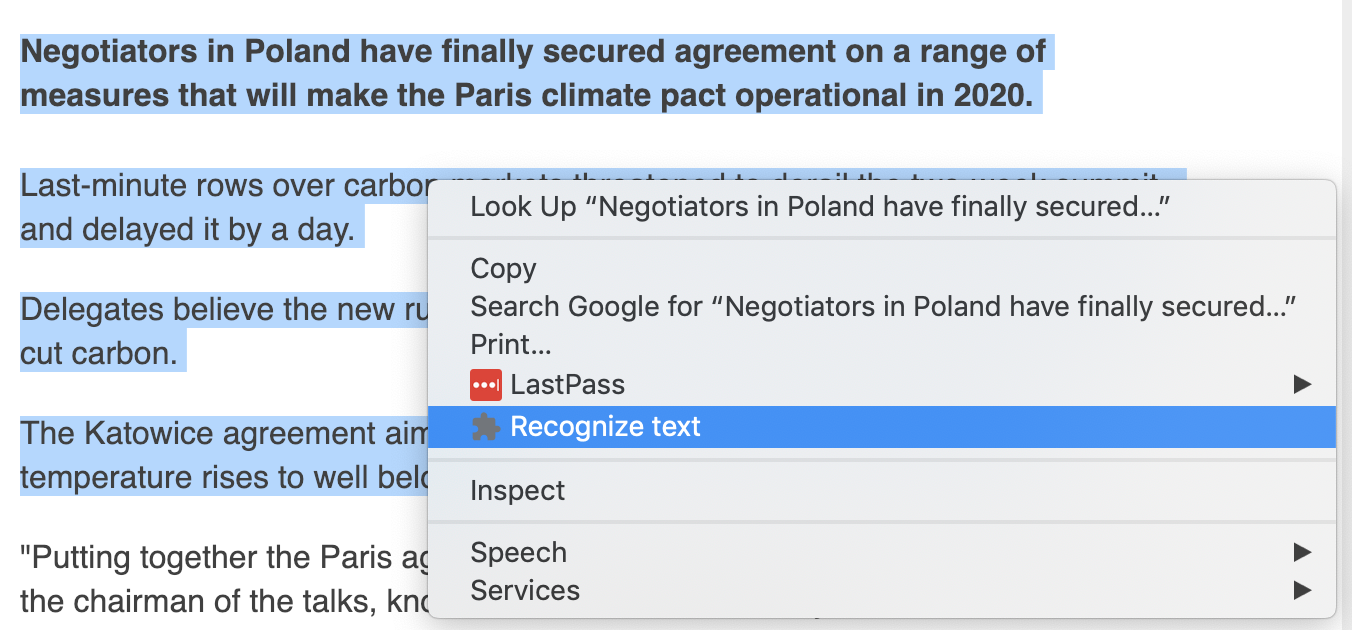
\includegraphics[width=10cm]{images/implementacja/context_menu.png}
    \caption{Menu kontekstowe}
    \end{figure}
    
    \item Options UI
    
    Definiuje stronę z ustawieniami dodatku. Do przechowywania konfiguracji w przeglądarce możemy użyć obiektu 'storage' dedykowanego dla dodatków przeglądarki Chrome - przed użyciem musimy umieścić go w liście 'permissions' pliku manifest. 
    
    \begin{figure}[H]
    \centering
    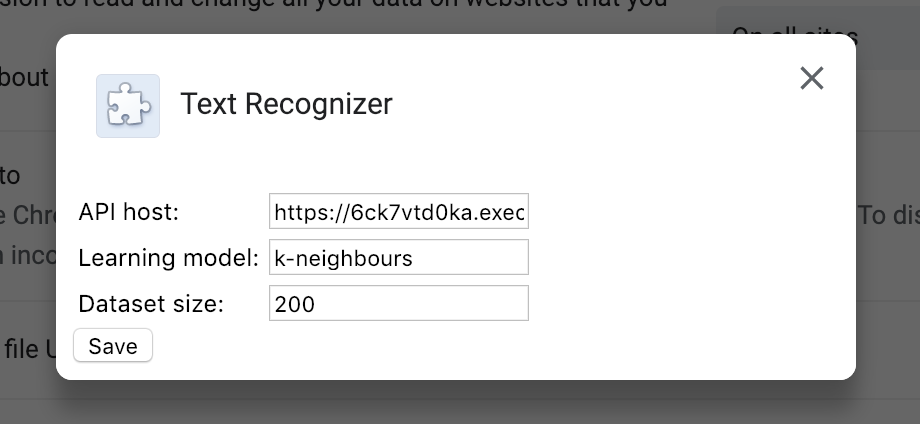
\includegraphics[width=10cm]{images/implementacja/options.png}
    \caption{Panel ustawień}
    \end{figure}
    
\newpage
\section{Architektura}

Wysokopoziomową budowę systemu można przedstawić za pomocą diagramu \ref{fig:architecture}. Warstwę prezentacji, za pomocą której użytkownik komunikuje się z systemem jest dodatek do przeglądarki Chrome. On natomiast używa zapytań HTTP do wymiany informacji z warstwą logiki aplikacji (Serwis klasyfikacji), której funkcję pełni aplikacja napisana w języku Python. Oprócz odpowiadania na żądania użytkownika ma on jeszcze dwie główne funkcjonalności - pobieranie danych z serwisów internetowych oraz zapisywanie ich oraz odczytywanie z warstwy persystencji danych, której rolę pełni DynamoDB.

    \begin{figure}[H]
    \centering
    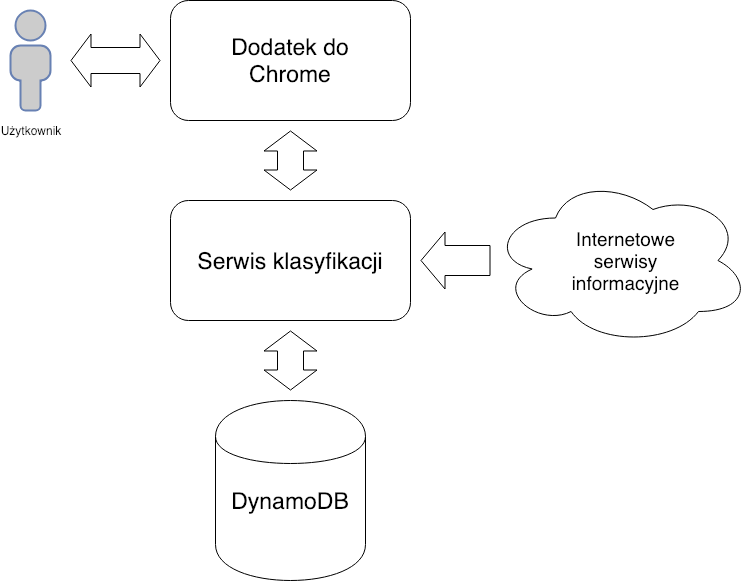
\includegraphics[width=12cm]{images/implementacja/architecture.png}
    \caption{Wysokopoziomowa architektura systemu}
    \label{fig:architecture}
    \end{figure}
    
\end{enumerate}
\chapter{Wdrożenie systemu w chmurze obliczeniowej}

Wyróżnia się kilka podstawowych etapów niezbędnych do prawidłowego wdrożenia systemu:

\begin{enumerate}
    \item Przygotowanie dokumentacji.
    \item Ustawienie infrastruktury.
    \item Przygotowanie środowiska testowego.
    \item Testy systemu.
    \item Migracja danych.
    \item Uruchomienie systemu produkcyjnego.
\end{enumerate}

W mojej pracy skupiłem się na dwóch punktach: ustawienia infrastruktury oraz przygotowania środowiska testowego. Zostało to zrealizowane w chmurze ze względu na redukcję kosztów oraz skalowalność rozwiązania. Nie wymaga to od dostawcy oprogramowania własnej infrastruktury oraz pozwala na sprawne zarządzanie posiadanymi zasobami.

System kategoryzacji korzysta z trzech usług zlokalizowanych na platformie Amazon Web Services:

\begin{enumerate}
    \item API gateway
    
    Bramka, która zajmuje się przyjmowaniem żądań użytkownika i przekazywanie ich do odpowiedniego serwisu. API Gateway w systemie klasyfikacji przyjmuje żądanie HTTP od użytkownika i przekazuje je do funkcji działającej w usłudze AWS Lambda.
    
    \item AWS Lambda
    
    Usługa pozwalająca na uruchamianie własnego kodu użytkownika w postaci funkcji. Uruchamianie może być wywołane ręcznie lub poprzez inny serwis AWS. W systemie klasyfikacji uruchomienie funkcji wywoływane jest przez serwis API Gateway.
    
    \item DynamoDB
    
    Baza danych zorientowana dokumentowo przechowywująca dane w postaci klucz-wartość. Obszerwnie opisana w rozdziale \ref{cha:wprowadzenieTechnologiczne}.
\end{enumerate}

\newpage
\begin{figure}[H]
    \centering
    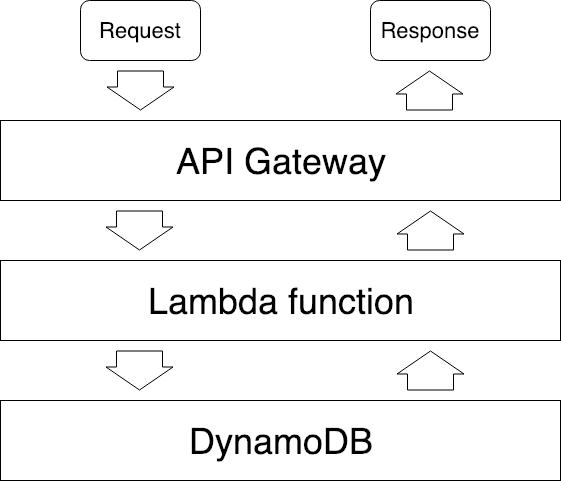
\includegraphics[width=10cm]{images/wdrozenie/aws_Architecture.png}
    \caption{Architektura infrastruktury systemu wdrożonego na platformie Amazon Web Services}
    \label{fig:architecture}
    \end{figure}

\section{AWS Lambda - wdrażanie aplikacji w środowisku serverless}

Lambda oferuje nam moc obliczeniową bez potrzeby dostarczania oraz zarządzania serwerami. Amazon dostarcza nam całe potrzebne środowisko - naszym zadaniem jest jedynie przekazanie kodu, który ma być uruchamiany. Za skalowanie oraz administrację środowiskiem odpowiedzialny jest dostawca usług.

Umieszczenie dużej aplikacji w usłudze AWS Lambda nie jest prostym wyzwaniem. Sporym ograniczeniem jest maksymalny rozmiar spakowanego kodu - 50MB. Serwis klasyfikacji z racji zależności z bibliotekami do obliczeń (numpy i scikit-learn) oraz zestawu słów do przetwarzania języka naturalnego osiąga ponad dwukrotnie większy rozmiar. 

Problemy z ograniczeniami usługi AWS Lambda rozwiązałem posługując się projektem Zappa \footnote{https://github.com/Miserlou/Zappa}. Pozwolił on na zautomatyzowanie następujących czynności:

\begin{enumerate}
    \item Spakowanie aplikacji wraz ze wszystkimi dependencjami kompatybilnymi ze środowiskiem AWS Lambda w plik zip.
    
    \item Utworzenie odpowiednich uprawnień do innych zasobów platformy AWS.
    
    \item Utworzenie funkcji AWS Lambda ze spakowanym kodem.
    
    \item Utworzenie API Gateway odpowiedzialnego za komunikację z funkcją AWS Lambda.
\end{enumerate}

Ograniczenie wielkości spakowanego kodu zostało ominięte dzięki opcji 'slim\_handler' \footnote{https://github.com/Miserlou/zappa-blog/blob/master/posts/slim-handler.md}. Gdy jej używamy - do funkcji AWS Lambda przekazywana jest jedynie minimalna ilość kodu, a reszta wysłana zostaje do serwisu AWS Simple Storage Service (S3) \footnote{https://aws.amazon.com/s3/}. Gdy następuje tzw. 'cold start', czyli pierwsze uruchomienie aplikacji na nowej maszynie - wtedy reszta kodu jest na nią pobierana do tymczasowej lokacji i wykonywana przy każdym odwołaniu z API Gateway. Wadą takiego rozwiązania jest wydłużony czas wykonywania pierwszego zapytania do API - wtedy właśnie reszta kodu musi zostać pobrana.

Dodatkowym aspektem wdrożenia projektu była integracja apikacji działającej w środowisku serverless z bazą danych. Aplikacja komunikuje się z bazą DynamoDB wykorzystując AWS SDK, jednak, aby korzystać z jej zasobów muszą zostać zdefiniowane odpowiednie uprawnienia. W konfiguracji projektu Zappa znalazły się one w sekcji 'extra\_permissions':

\begin{verbatim}
    "extra_permissions": [
      {
        "Effect": "Allow",
        "Action": [
          "dynamodb:DeleteItem",
          "dynamodb:GetItem",
          "dynamodb:PutItem",
          "dynamodb:UpdateItem",
          "dynamodb:Scan",
          "dynamodb:Query",
          "dynamodb:ListTables",
          "dynamodb:CreateTable",
          "dynamodb:DeleteTable",
          "dynamodb:UpdateTable"
        ],
        "Resource": "*"
      }
    ]
\end{verbatim}

Wpis ten definiuje dostęp do operacji zarządzania tabelami oraz do wszelkich operacji CRUD (Tworzenie, odczyt, modyfikacja oraz usuwanie rekordów). Symbol '*' odpowiada wszystkim zasobom w ramach jednego konta na platformie AWS.




\chapter{Walidacja rezultatów}
\label{cha:walidacja}

Pomimo, że testy oraz skuteczność poszczególnych klasyfikatorów zostały przedstawione w rozdziale \ref{cha:analizaDanych}, to wciąż nie można było ocenić jak system klasyfikacji zachowa się przy użyciu faktycznych danych wprowadzonych przez użytkownika. Z tego powodu w tym rozdziale opisano testy przeprowadzone przy użyciu rzeczywistych danych.

Testy przeprowadziłem bazując na artykułach ze strony BBC News\footnote{https://www.bbc.com/news} oraz BBC Sport \footnote{https://www.bbc.com/sport}. W zbiorze danych uczących nie znalazły się żadne artykuły z tych serwisów, więc wyniki testów powinny być obiektywne.

\section{Założenia}

\subsection{Zbiór uczący}

W zbiorze uczącym znalazło się 5000 artykułów z poszczególnych kategorii:

\begin{enumerate}
    \item Biznes.
    \item Sport.
    \item Rozrywka.
    \item Polityka.
    \item Technologia.
\end{enumerate}

Zbiór zawierał po 500 artykułów z każdej wymienionej kategorii, z czego każdy artykuł miał około 60 słów. W opcjach aplikacji możliwy był wybór jednego z trzech algorytmów: naiwny klasyfikator bayesowski, metoda wektorów nośnych oraz algorytm K najbliższych sąsiadów. Jesteśmy również w stanie zdefiniować rozmiar zbioru jaki zostanie użyty w uczenia algorytmu (maksymalnie 2500 elementów).

Przed uczeniem algorytmu dane są wstępnie przetwarzane metodami opisanymi w rozdziale \ref{cha:analizaDanych} oraz sprowadzane do modelu TF-IDF.

\subsection{Zbiór testowy}

W zbiorze testowym znalazło się 93 artykuły ze strony BBC News. Wszystkie artykuły pochodziły z kategorii takich samych lub analogicznych do kategorii artykułów ze zbioru uczącego. Zbiór zawierał po 40 artykułów o polityce, sporcie oraz technologii, 39 artykułów o rozrywce oraz 34 biznesowych artykułów. Łącznie w każdym teście zostały klasyfikowane 193 artykuły.

\section{Metodologia}

Do przeprowadzenia testów serwisu klasyfikacji napisałem skrypt wykonujący testy typu 'end-to-end', czyli testujące całą aplikację, nie tylko poszczególne komponenty. Pomijany jest jedynie interfejs użytkownika. Skrypt testujący pobiera dane z pliku JSON, który ma strukturę listy z której każdy element odzwierciedla jeden przypadek testowy. Następnie wykonywane jest zapytanie REST do serwisu i uzyskany wynik porównywany jest do oczekiwanego (zdefiniowanego w pliku z danymi testowymi).

Jako parametry pojedynczego testu podany zostanie jeden algorytm (klasyfikator bayesowski, metoda wektorów nośnych lub algorytm k najbliższych sąsiadów) oraz ilość danych w zbiorze uczącym (10, 50, 100, 200, 500, 1000 lub 2000 elementów). Zostanie również zmierzony czas przeprowadzenia testu. Pozwoli to wybrać optymalny algorytm oraz ilość danych. Plik wejściowy z danymi do testu oraz plik wyjściowy z wynikiem testu są w formacie JSON.

Przykładowy plik testowy:

\begin{verbatim}
[
  {
    "content": "US financial markets were mixed on F...",
    "label": "business"
  },
  {
    "content": "Evidence that adverts for major brands...",
    "label": "technology"
  }
]
\end{verbatim}

Przykładowy rezultat testu:

\begin{verbatim}
{
  'fail_info': [
    {
      'actual_label': 'technology',
      'content': 'US financial markets were mixed on Friday after a ',
      'expected_label': 'business'
    }
  ],
  'failed': 1,
  'passed': 1,
  'test_cases': 2,
  'test_params': {
    'dataset_size': 30,
    'model': 'naive-bayes'
  }
}
\end{verbatim}

\section{Klasyfikacja całych artykułów}

W pierwszym teście będę klasyfikował artykuły w całości - jako wejście aplikacji zostanie podana cała zawartość wybranego tekstu. Wynik odzwierciedla jaka część artykułów została sklasyfikowana poprawnie (np. 80\% oznacza, że 8 na 10 artykułom została przypisana odpowiednia kategoria).

Warty zauważenia jest fakt, że dysponujemy pięcioma kategoriami w zbiorze testowym - algorytm losujący kategorie powinien osiągać skuteczność około 20\%.

\begin{center}
\begin{longtable}{ |l|l|l|l| } 
 \hline
 Algorytm & Rozmiar zbioru uczącego & Wynik & Czas wykonania testu \\ 
 \hline
 naiwny klasyfikator bayesowski & 10    & 46.11\% & 61s\\
 naiwny klasyfikator bayesowski & 50    & 64.25\% & 58s\\
 naiwny klasyfikator bayesowski & 100   & 75.65\% & 59s\\
 naiwny klasyfikator bayesowski & 200   & 74.09\% & 68s\\
 naiwny klasyfikator bayesowski & 500   & 78.24\% & 105s\\
 naiwny klasyfikator bayesowski & 1000  & 75.13\% & 172s\\
 naiwny klasyfikator bayesowski & 2000  & 76.68\% & 296s\\
\hline
 metoda wektorów nośnych & 10   & 36.27\% & 44s\\
 metoda wektorów nośnych & 50   & 50.78\% & 49s\\
 metoda wektorów nośnych & 100  & 48.70\% & 57s\\
 metoda wektorów nośnych & 200  & 51.81\% & 72s\\
 metoda wektorów nośnych & 500  & 54.40\% & 128s\\
 metoda wektorów nośnych & 1000 & 51.81\% & 261s\\
 metoda wektorów nośnych & 2000 & 55.96\% & 704s\\
\hline
 k najbliższych sąsiadów & 10   & 33.68\% & 50s\\
 k najbliższych sąsiadów & 50   & 56.48\% & 63s\\
 k najbliższych sąsiadów & 100  & 61.14\% & 58s\\
 k najbliższych sąsiadów & 200  & 67.88\% & 69s\\
 k najbliższych sąsiadów & 500  & 67.88\% & 106s\\
 k najbliższych sąsiadów & 1000 & 70.98\% & 169s\\
 k najbliższych sąsiadów & 2000 & 70.47\% & 337s\\
 \hline
\end{longtable}
\end{center}

Najlepsze wyniki aplikacja osiągnęła stosując naiwny klasyfikator bayesowski. Już przy danych uczących w ilości 100 elementów ponad 3 na 4 artykuły zostały sklasyfikowane poprawnie.
W metodzie wektorów nośnych oraz klasyfikatorze bayesowskim przy zbiorach danych większym niż 500 elementów nastąpiło pogorszenie wyniku - mamy tu do czynienia ze zjawiskiem nadmiernego dopasowania (ang. overfitting) \footnote{https://pl.wikipedia.org/wiki/Nadmierne_dopasowanie}, czyli model zbyt dobrze dopasowuje się do danych uczących przez co osiąga na nich dobre wyniki, ale radzi sobie dużo gorzej z danymi spoza zbiorów uczących.

\section{Klasyfikacja części artykułów}

Kolejny test zostanie przeprowadzony jedynie na części tekstu. Z każdego artykułu w powyższym teście zostały wycięte 3 zdania, które zostaną poddane klasyfikacji. Wyniki prezentują się następująco:

\begin{center}
\begin{longtable}{ |l|l|l|l| } 
 \hline
 Algorytm & Rozmiar zbioru uczącego & Wynik & Czas wykonania testu \\ 
 \hline
 naiwny klasyfikator bayesowski & 10    & 43.52\% & 51s\\
 naiwny klasyfikator bayesowski & 50    & 66.84\% & 63s\\
 naiwny klasyfikator bayesowski & 100   & 66.84\% & 60s\\
 naiwny klasyfikator bayesowski & 200   & 68.91\% & 78s\\
 naiwny klasyfikator bayesowski & 500   & 76.17\% & 116s\\
 naiwny klasyfikator bayesowski & 1000  & 76.68\% & 181s\\
 naiwny klasyfikator bayesowski & 2000  & 78.24\% & 324s\\
\hline
 metoda wektorów nośnych & 10   & 41.45\% & 48s\\
 metoda wektorów nośnych & 50   & 50.78\% & 54s\\
 metoda wektorów nośnych & 100  & 54.92\% & 64s\\
 metoda wektorów nośnych & 200  & 51.30\% & 107s\\
 metoda wektorów nośnych & 500  & 53.37\% & 139s\\
 metoda wektorów nośnych & 1000 & 48.70\% & 283s\\
 metoda wektorów nośnych & 2000 & 54.40\% & 695s\\
\hline
 k najbliższych sąsiadów & 10   & 34.20\% & 47s\\
 k najbliższych sąsiadów & 50   & 58.03\% & 53s\\
 k najbliższych sąsiadów & 100  & 62.18\% & 60s\\
 k najbliższych sąsiadów & 200  & 64.77\% & 105s\\
 k najbliższych sąsiadów & 500  & 64.77\% & 113s\\
 k najbliższych sąsiadów & 1000 & 66.84\% & 194s\\
 k najbliższych sąsiadów & 2000 & 71.50\% & 330s\\
 \hline
\end{longtable}
\end{center}

Powyższe wyniki dowodzą, że nie potrzebujemy całej treści artykułu, aby móc określić jego kategorię. Analizując jedynie części tekstu (w tym wypadku 3 losowo wybrane zdania) możemy stwierdzić, że wybrany fragment jest klasyfikowany z bardzo podobnym rezultatem co jego całość.
\chapter{Podsumowanie}
\label{cha:podsumowanie}

Badania oraz aplikacja wykonana w ramach tej pracy dowiodły, że wykorzystanie metod nauczania maszynowego do klasyfikacji języka naturalnego w formie danych tekstowych przynosi oczekiwane rezultaty. Zastosowane algorytmy są w stanie wspierać człowieka oraz automatyzować jego pracę w związku z przetwarzaniem dużej ilości danych.


W ramach pracy udało się rozwinąć system, który jest w stanie przetwarzać i kategoryzować dane w formie tekstu napisanego za pomocą języka naturalnego. Zaproponowane rozwiązanie wyróżnia się dużymi możliwościami konfiguracji. W pracy wykorzystałem dane pochodzące z serwisów informacyjnych, pogrupowane według tematyki, której dotyczą. Możemy jednak dostarczyć własne dane opisane kategoriami, które chcemy uzyskać jako wynik działania programu - wtedy system będzie klasyfikował tekst bazując na dostarczonych zbiorach danych. Dodatkową możliwością jest wybór algorytmu oraz ilość danych uczących, tak aby skuteczność i szybkość działania były optymalne dla potrzeb użytkownika.

Kolejną mocną stroną rozwiniętego systemu klasyfikacji jest prosty interfejs, który może być użyty przez użytkowników bez wiedzy technicznej. Zazwyczaj oprogramowanie tego typu jest przeznaczone dla programistów i wymaga ono integracji z własnym programami. Tutaj natomiast możliwa jest interakcja poprzez przeglądarkę bezpośrednio z treściami dostępnymi na stronach internetowych, dzięki czemu poprawnie skonfigurowany i wdrożony system klasyfikacji jest dostępny dla każdego użytkownika. Serwis klasyfikacji posiada również całą funkcjonalność dostępną poprzez protokół HTTP. Daje nam to możliwość zastosowania serwisu w istniejących już aplikacjach.

System kategoryzacji wymaga konfiguracji parametrów algorytmu uczącego za każdym wywołaniem. Użytkownik powinien mieć możliwość automatycznego wyboru algorytmu, który najlepiej sprawdzi się na jego danych. Wstępne przetwarzanie danych oraz reprezentacja numeryczna tekstu oparte zostały na podstawowych metodach, przez co znaczna część informacji z tekstu jest tracona. Gdyby zostały użyte bardziej złożone techniki - rezultaty powinny być lepsze.

W przyszłości aplikacja powinna być rozwinięta pod względem interakcji z użytkownikiem. Obecny interfejs w postaci dodatku do przeglądarki Chrome jest wygodny w kontekście kategoryzacji danych znajdujących się bezpośrednio na stronach internetowych, lecz nie powala na przetwarzanie dużych ilości danych znajdujących się w plikach, lub w innych źródłach.

Kolejnym elementem, który powinien być dalej rozwijany jest klasyfikacja danych w wielu wymiarach. Aplikacja powinna przypisywać do tekstu wiele kategorii (np. rodzaj tekstu, użyty język, wyrażane emocje), które pozwoliłyby na bardziej precyzyjny opis danych.


% itd.
% \appendix
% \include{dodatekA}
% \include{dodatekB}
% itd.

\nocite{*}
\printbibliography

\end{document}
